\chapter{Notes}
\section{extra refs}


\subsection{Introduction synapses}
\textcolor{red}{review}
@article{humeau2019next,
  title={The next generation of approaches to investigate the link between synaptic plasticity and learning},
  author={Humeau, Yann and Choquet, Daniel},
  journal={Nature neuroscience},
  volume={22},
  number={10},
  pages={1536--1543},
  year={2019},
  publisher={Nature Publishing Group}
}

\subsection{centrality measures}
@article{valente2008correlated,
  title={How correlated are network centrality measures?},
  author={Valente, Thomas W and Coronges, Kathryn and Lakon, Cynthia and Costenbader, Elizabeth},
  journal={Connections (Toronto, Ont.)},
  volume={28},
  number={1},
  pages={16},
  year={2008},
  publisher={NIH Public Access}
}

@inproceedings{koschutzki2004comparison,
  title={Comparison of centralities for biological networks},
  author={Kosch{\"u}tzki, Dirk and Schreiber, Falk},
  booktitle={German Conference on Bioinformatics 2004, GCB 2004},
  year={2004},
  organization={Gesellschaft f{\"u}r Informatik eV}
}

@article{jalili2016evolution,
  title={Evolution of centrality measurements for the detection of essential proteins in biological networks},
  author={Jalili, Mahdi and Salehzadeh-Yazdi, Ali and Gupta, Shailendra and Wolkenhauer, Olaf and Yaghmaie, Marjan and Resendis-Antonio, Osbaldo and Alimoghaddam, Kamran},
  journal={Frontiers in Physiology},
  volume={7},
  pages={375},
  year={2016},
  publisher={Frontiers}
}

\subsection{communities}
\textcolor{red}{Over 1000 citations}
@article{porter2009communities,
  title={Communities in networks},
  author={Porter, Mason A and Onnela, Jukka-Pekka and Mucha, Peter J},
  journal={Notices of the AMS},
  volume={56},
  number={9},
  pages={1082--1097},
  year={2009}
}

\textcolor{red}{cited by 853}
@article{good2010performance,
  title={Performance of modularity maximization in practical contexts},
  author={Good, Benjamin H and De Montjoye, Yves-Alexandre and Clauset, Aaron},
  journal={Physical Review E},
  volume={81},
  number={4},
  pages={046106},
  year={2010},
  publisher={APS}
}

\textcolor{red}{citations 97}
@article{lewis2010function,
  title={The function of communities in protein interaction networks at multiple scales},
  author={Lewis, Anna CF and Jones, Nick S and Porter, Mason A and Deane, Charlotte M},
  journal={BMC systems biology},
  volume={4},
  number={1},
  pages={100},
  year={2010},
  publisher={Springer}
}

\textcolor{red}{cited by 8635}
@article{fortunato2010community,
  title={Community detection in graphs},
  author={Fortunato, Santo},
  journal={Physics reports},
  volume={486},
  number={3-5},
  pages={75--174},
  year={2010},
  publisher={Elsevier}
}

\textcolor{red}{cited by 457}
@article{lancichinetti2012consensus,
  title={Consensus clustering in complex networks},
  author={Lancichinetti, Andrea and Fortunato, Santo},
  journal={Scientific reports},
  volume={2},
  pages={336},
  year={2012},
  publisher={Nature Publishing Group}
}

\textcolor{red}{cited by 877}
@article{lancichinetti2011finding,
  title={Finding statistically significant communities in networks},
  author={Lancichinetti, Andrea and Radicchi, Filippo and Ramasco, Jos{\'e} J and Fortunato, Santo},
  journal={PloS one},
  volume={6},
  number={4},
  year={2011},
  publisher={Public Library of Science}
}

\subsection{multilayer networks}@article{humeau2019next,
  title={The next generation of approaches to investigate the link between synaptic plasticity and learning},
  author={Humeau, Yann and Choquet, Daniel},
  journal={Nature neuroscience},
  volume={22},
  number={10},
  pages={1536--1543},
  year={2019},
  publisher={Nature Publishing Group}
}

\textcolor{red}{cited by 1936}
@article{kivela2014multilayer,
  title={Multilayer networks},
  author={Kivel{\"a}, Mikko and Arenas, Alex and Barthelemy, Marc and Gleeson, James P and Moreno, Yamir and Porter, Mason A},
  journal={Journal of complex networks},
  volume={2},
  number={3},
  pages={203--271},
  year={2014},
  publisher={Oxford University Press}
}

\textcolor{red}{over 100 pages, cited by 1878}
@article{boccaletti2014structure,
  title={The structure and dynamics of multilayer networks},
  author={Boccaletti, Stefano and Bianconi, Ginestra and Criado, Regino and Del Genio, Charo I and G{\'o}mez-Gardenes, Jes{\'u}s and Romance, Miguel and Sendina-Nadal, Irene and Wang, Zhen and Zanin, Massimiliano},
  journal={Physics Reports},
  volume={544},
  number={1},
  pages={1--122},
  year={2014},
  publisher={Elsevier}
}

New has modularity of real world networks

@article{zhang2009big,
  title={A big world inside small-world networks},
  author={Zhang, Zhihua and Zhang, Jianzhi},
  journal={PloS one},
  volume={4},
  number={5},
  year={2009},
  publisher={Public Library of Science}
}

cited by 1044

@article{brandes2007modularity,
  title={On modularity clustering},
  author={Brandes, Ulrik and Delling, Daniel and Gaertler, Marco and Gorke, Robert and Hoefer, Martin and Nikoloski, Zoran and Wagner, Dorothea},
  journal={IEEE transactions on knowledge and data engineering},
  volume={20},
  number={2},
  pages={172--188},
  year={2007},
  publisher={IEEE}
}

\subsection{general notes}
Wagner and Fell small world

\subsection{extra results}
Enrichment of new graph components


 MEAN SAMPLE\ SIZE = 250000
 TOTAL GENES = 18673
 CONDITIONED INTERNAL = genesize, log genesize, genedensity, log genedensity, inverse mac, log inverse mac
SET           NGENES       BETA   BETA STD         SE            P
new in graph    1397     0.0553     0.0145     0.0293     0.029806
new graph       4414      0.101     0.0427     0.0186   3.1989e-08
PSD             3414      0.113     0.0436     0.0201   1.0565e-08



\section{Readme from Sniekers}
\label{sec:notes readme from sniekers}

Uses NCBI 37.3 in MAGMA

     Association results of the meta-analysis for intelligence based on 78,308 individuals in 13 cohorts. 
     Version date: 10-07-2017

  Columns:
Chromosome: chromosome number
position: base pair position of the SNP on the chromosome (reported on GRCh37)
rsid: SNP rs number
ref: effect allele
alt: non-effect allele
N: sample size
MAF: minor allele frequency in UK Biobank
Beta: effect size of the effect allele
SE: standard error of the effect
Zscore: Z-score computed in METAL by a weighted Z-score method
p   value: P-value computed in METAL by a weighted Z-score method
direction: direction of the effect in each of the cohorts, order: CHIC (consisting of 6 cohorts), UKB-wb, UKB-ts, ERF, GENR, HU, MCTFR, STR

Beta/SE were calculated from METAL Z-scores using the formula from Zhu et al (Nature Genetics, 2016):

Beta = Zscore / sqrt( 2 * MAF * ( 1 - MAF) * ( N + $Zscore^2$ ) )
SE = 1 / sqrt( 2 * MAF * ( 1 - MAF ) * ( N + $Zscore^2$ ) )

\section{Useful papers for methods}

MDD for quoting MAGMA \url{https://www.nature.com/articles/s41467-018-03819-3}

\section{Community detection}

Communities allow the network to be broken up into smaller components which can be analysed in turn and which may represent functional units.


\section{Modularity}
\label{sec:modularity definition}

for an adjacency matrix $A_{ij}$ we want to know how many edges pass between similar nodes that share a property be it an ontology term or a community membership.

Total number of edges is between nodes of same group is:

\begin{equation}
\label{eq:notes_modularity_totaledges}
    \frac{1}{2} \sum_{i,j} A_{i,j}\delta_{g_i g_j}
\end{equation}

The expected number of edges between all nodes of the same type is 

\begin{equation}
    \frac{1}{2}\sum_{i,j} \frac{k_i k_j}{2m}\delta_{g_i g_j}
\end{equation}

The modularity Q is 

\begin{equation}
    Q=\frac{1}{2m}\sum_{i,j}\textcolor{red}{(A_{i,j}-\frac{k_i k_j}{2m}}) \delta{g_i g_j}
\end{equation}

The red term is:

\begin{equation}
    B_{ij} = \sum_{i,j} A_{i,j} - \frac{k_i k_j}{2m}
\end{equation}

$\mathbf{B}$ is the modularity matrix which is n by n having elements $B_{i,j}$

\section{Simple example of spectral graph partitioning}
\label{sec:simple example of spectral graph partitioning}

Using the first eigenvector of the modularity matrix results in a partition with modularity 0.21. The distribution of the first four eigenvectors can be seen in figure~\ref{fig:simple example of spectral clustering}.\todo{?remove size for fourth}

Gene ontology analysis shows that the groups are quite different one of 1111 members linked to mRNA processing and biosynthesis see tables~\ref{tab:1111 group generated from sign of first eigenvector of modularity matrix. Biological function} compared with the genome and \ref{tab:1111 group generated from sign of first eigenvector of modularity matrix background PSP. Biological function. Alpha = 5.22520639565263e-06} compared with the rest of the PSP. The other group is of 2346 genes linked to trans-synaptic signalling see tables~\ref{tab:2346 group generated from sign of first eigenvector of modularity matrix. Biological function} and with background of PSP genes ~\ref{tab:2346 group generated from sign of first eigenvector of modularity matrix background PSP. Biological function. Alpha = 5.22520639565263e-06}
\begin{figure}
    \centering
    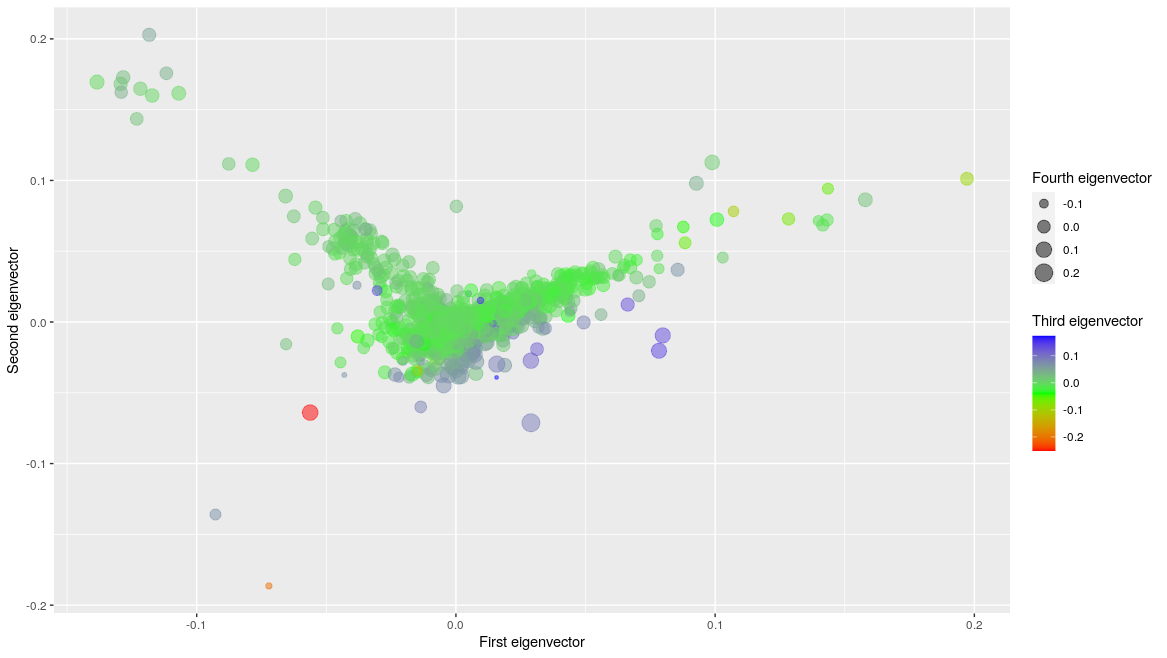
\includegraphics[width=\textwidth]{images/Rplot_eigenvectors_of_PSP_modularity_matrix.png}
    \caption{Simple example of spectral clustering of the PSP. The values of the $i$th entries of the first and second eigenvector are plotted on the x axis.}
    \label{fig:simple example of spectral clustering}
\end{figure}

% Sat May 16 14:53:46 2020
\begin{table}[ht]
\centering
\begin{tabular}{llrrrr}
  \hline
GO.ID & Term & Annotated & Significant & Expected & classic \\ 
  \hline
GO:0034641 & cellular nitrogen compound metabolic pro... & 1208 & 621 & 393.5 & $1.00 \times 10^{-30}$ \\ 
  GO:0016071 & mRNA metabolic process & 254 & 210 & 82.7 & $1.00 \times 10^{-30}$ \\ 
  GO:0010467 & gene expression & 922 & 506 & 300.3 & $1.00 \times 10^{-30}$ \\ 
  GO:0090304 & nucleic acid metabolic process & 801 & 452 & 260.9 & $1.00 \times 10^{-30}$ \\ 
  GO:0044271 & cellular nitrogen compound biosynthetic ... & 900 & 490 & 293.2 & $1.00 \times 10^{-30}$ \\ 
  GO:0043604 & amide biosynthetic process & 297 & 225 & 96.8 & $1.00 \times 10^{-30}$ \\ 
  GO:0006412 & translation & 258 & 204 & 84.0 & $1.00 \times 10^{-30}$ \\ 
  GO:0043043 & peptide biosynthetic process & 262 & 205 & 85.3 & $1.00 \times 10^{-30}$ \\ 
  GO:0034645 & cellular macromolecule biosynthetic proc... & 803 & 447 & 261.6 & $1.00 \times 10^{-30}$ \\ 
  GO:0009059 & macromolecule biosynthetic process & 830 & 456 & 270.4 & $1.00 \times 10^{-30}$ \\ 
  GO:0046483 & heterocycle metabolic process & 1076 & 549 & 350.5 & $1.00 \times 10^{-30}$ \\ 
  GO:0006139 & nucleobase-containing compound metabolic... & 1050 & 537 & 342.0 & $1.00 \times 10^{-30}$ \\ 
  GO:0016070 & RNA metabolic process & 716 & 407 & 233.2 & $1.00 \times 10^{-30}$ \\ 
  GO:1901360 & organic cyclic compound metabolic proces... & 1121 & 562 & 365.2 & $1.00 \times 10^{-30}$ \\ 
  GO:0006725 & cellular aromatic compound metabolic pro... & 1088 & 549 & 354.4 & $1.00 \times 10^{-30}$ \\ 
  GO:0006401 & RNA catabolic process & 179 & 152 & 58.3 & $1.00 \times 10^{-30}$ \\ 
  GO:0006402 & mRNA catabolic process & 175 & 149 & 57.0 & $1.00 \times 10^{-30}$ \\ 
  GO:1901576 & organic substance biosynthetic process & 1147 & 564 & 373.6 & $1.00 \times 10^{-30}$ \\ 
  GO:0009058 & biosynthetic process & 1160 & 568 & 377.9 & $1.00 \times 10^{-30}$ \\ 
  GO:0043603 & cellular amide metabolic process & 368 & 248 & 119.9 & $1.00 \times 10^{-30}$ \\ 
   \hline
\end{tabular}
\caption{1111 group generated from sign of first eigenvector of modularity matrix. Biological function} 
\label{tab:1111 group generated from sign of first eigenvector of modularity matrix. Biological function}
\end{table}

% latex table generated in R 3.6.3 by xtable 1.8-4 package
% Sat May 16 14:55:07 2020
\begin{table}[ht]
\centering
\begin{tabular}{llrrrr}
  \hline
GO.ID & Term & Annotated & Significant & Expected & classic \\ 
  \hline
GO:0030030 & cell projection organization & 572 & 483 & 385.7 & $7.80 \times 10^{-24}$ \\ 
  GO:0120036 & plasma membrane bounded cell projection ... & 566 & 478 & 381.6 & $1.40 \times 10^{-23}$ \\ 
  GO:0099537 & trans-synaptic signaling & 316 & 281 & 213.1 & $1.30 \times 10^{-20}$ \\ 
  GO:0023052 & signaling & 1510 & 1142 & 1018.1 & $1.50 \times 10^{-20}$ \\ 
  GO:0007268 & chemical synaptic transmission & 310 & 276 & 209.0 & $2.00 \times 10^{-20}$ \\ 
  GO:0098916 & anterograde trans-synaptic signaling & 310 & 276 & 209.0 & $2.00 \times 10^{-20}$ \\ 
  GO:0007154 & cell communication & 1508 & 1140 & 1016.8 & $2.30 \times 10^{-20}$ \\ 
  GO:0099536 & synaptic signaling & 318 & 282 & 214.4 & $2.90 \times 10^{-20}$ \\ 
  GO:0051049 & regulation of transport & 623 & 511 & 420.1 & $2.10 \times 10^{-19}$ \\ 
  GO:0007399 & nervous system development & 772 & 617 & 520.5 & $2.20 \times 10^{-18}$ \\ 
  GO:0048666 & neuron development & 439 & 368 & 296.0 & $9.30 \times 10^{-17}$ \\ 
  GO:0030029 & actin filament-based process & 333 & 287 & 224.5 & $1.70 \times 10^{-16}$ \\ 
  GO:0030036 & actin cytoskeleton organization & 284 & 249 & 191.5 & $2.10 \times 10^{-16}$ \\ 
  GO:0050804 & modulation of chemical synaptic transmis... & 218 & 197 & 147.0 & $2.20 \times 10^{-16}$ \\ 
  GO:0031175 & neuron projection development & 404 & 340 & 272.4 & $5.30 \times 10^{-16}$ \\ 
  GO:0099177 & regulation of trans-synaptic signaling & 219 & 197 & 147.7 & $7.50 \times 10^{-16}$ \\ 
  GO:0032879 & regulation of localization & 853 & 667 & 575.1 & $1.20 \times 10^{-15}$ \\ 
  GO:0032989 & cellular component morphogenesis & 453 & 375 & 305.4 & $3.00 \times 10^{-15}$ \\ 
  GO:0030182 & neuron differentiation & 478 & 393 & 322.3 & $5.10 \times 10^{-15}$ \\ 
  GO:0048699 & generation of neurons & 515 & 420 & 347.2 & $7.00 \times 10^{-15}$ \\ 
   \hline
\end{tabular}
\caption{2346 group generated from sign of first eigenvector of modularity matrix. Biological function} 
\label{tab:2346 group generated from sign of first eigenvector of modularity matrix. Biological function}
\end{table}

% latex table generated in R 3.6.3 by xtable 1.8-4 package
% Sat May 16 14:59:26 2020
\begin{table}[ht]
\centering
\begin{tabular}{llrrrr}
  \hline
GO.ID & Term & Annotated & Significant & Expected & classic \\ 
  \hline
GO:0030030 & cell projection organization & 572 & 483 & 385.7 & $7.80 \times 10^{-24}$ \\ 
  GO:0120036 & plasma membrane bounded cell projection ... & 566 & 478 & 381.6 & $1.40 \times 10^{-23}$ \\ 
  GO:0099537 & trans-synaptic signaling & 316 & 281 & 213.1 & $1.30 \times 10^{-20}$ \\ 
  GO:0023052 & signaling & 1510 & 1142 & 1018.1 & $1.50 \times 10^{-20}$ \\ 
  GO:0007268 & chemical synaptic transmission & 310 & 276 & 209.0 & $2.00 \times 10^{-20}$ \\ 
  GO:0098916 & anterograde trans-synaptic signaling & 310 & 276 & 209.0 & $2.00 \times 10^{-20}$ \\ 
  GO:0007154 & cell communication & 1508 & 1140 & 1016.8 & $2.30 \times 10^{-20}$ \\ 
  GO:0099536 & synaptic signaling & 318 & 282 & 214.4 & $2.90 \times 10^{-20}$ \\ 
  GO:0051049 & regulation of transport & 623 & 511 & 420.1 & $2.10 \times 10^{-19}$ \\ 
  GO:0007399 & nervous system development & 772 & 617 & 520.5 & $2.20 \times 10^{-18}$ \\ 
  GO:0048666 & neuron development & 439 & 368 & 296.0 & $9.30 \times 10^{-17}$ \\ 
  GO:0030029 & actin filament-based process & 333 & 287 & 224.5 & $1.70 \times 10^{-16}$ \\ 
  GO:0030036 & actin cytoskeleton organization & 284 & 249 & 191.5 & $2.10 \times 10^{-16}$ \\ 
  GO:0050804 & modulation of chemical synaptic transmis... & 218 & 197 & 147.0 & $2.20 \times 10^{-16}$ \\ 
  GO:0031175 & neuron projection development & 404 & 340 & 272.4 & $5.30 \times 10^{-16}$ \\ 
  GO:0099177 & regulation of trans-synaptic signaling & 219 & 197 & 147.7 & $7.50 \times 10^{-16}$ \\ 
  GO:0032879 & regulation of localization & 853 & 667 & 575.1 & $1.20 \times 10^{-15}$ \\ 
  GO:0032989 & cellular component morphogenesis & 453 & 375 & 305.4 & $3.00 \times 10^{-15}$ \\ 
  GO:0030182 & neuron differentiation & 478 & 393 & 322.3 & $5.10 \times 10^{-15}$ \\ 
  GO:0048699 & generation of neurons & 515 & 420 & 347.2 & $7.00 \times 10^{-15}$ \\ 
   \hline
\end{tabular}
\caption{2346 group generated from sign of first eigenvector of modularity matrix background PSP. Biological function. Alpha = 5.22520639565263e-06} 
\label{tab:2346 group generated from sign of first eigenvector of modularity matrix background PSP. Biological function. Alpha = 5.22520639565263e-06}
\end{table}

% latex table generated in R 3.6.3 by xtable 1.8-4 package
% Sat May 16 15:00:11 2020
\begin{table}[ht]
\centering
\begin{tabular}{llrrrr}
  \hline
GO.ID & Term & Annotated & Significant & Expected & classic \\ 
  \hline
GO:0034641 & cellular nitrogen compound metabolic pro... & 1208 & 621 & 393.5 & $1.00 \times 10^{-30}$ \\ 
  GO:0016071 & mRNA metabolic process & 254 & 210 & 82.7 & $1.00 \times 10^{-30}$ \\ 
  GO:0010467 & gene expression & 922 & 506 & 300.3 & $1.00 \times 10^{-30}$ \\ 
  GO:0090304 & nucleic acid metabolic process & 801 & 452 & 260.9 & $1.00 \times 10^{-30}$ \\ 
  GO:0044271 & cellular nitrogen compound biosynthetic ... & 900 & 490 & 293.2 & $1.00 \times 10^{-30}$ \\ 
  GO:0043604 & amide biosynthetic process & 297 & 225 & 96.8 & $1.00 \times 10^{-30}$ \\ 
  GO:0006412 & translation & 258 & 204 & 84.0 & $1.00 \times 10^{-30}$ \\ 
  GO:0043043 & peptide biosynthetic process & 262 & 205 & 85.3 & $1.00 \times 10^{-30}$ \\ 
  GO:0034645 & cellular macromolecule biosynthetic proc... & 803 & 447 & 261.6 & $1.00 \times 10^{-30}$ \\ 
  GO:0009059 & macromolecule biosynthetic process & 830 & 456 & 270.4 & $1.00 \times 10^{-30}$ \\ 
  GO:0046483 & heterocycle metabolic process & 1076 & 549 & 350.5 & $1.00 \times 10^{-30}$ \\ 
  GO:0006139 & nucleobase-containing compound metabolic... & 1050 & 537 & 342.0 & $1.00 \times 10^{-30}$ \\ 
  GO:0016070 & RNA metabolic process & 716 & 407 & 233.2 & $1.00 \times 10^{-30}$ \\ 
  GO:1901360 & organic cyclic compound metabolic proces... & 1121 & 562 & 365.2 & $1.00 \times 10^{-30}$ \\ 
  GO:0006725 & cellular aromatic compound metabolic pro... & 1088 & 549 & 354.4 & $1.00 \times 10^{-30}$ \\ 
  GO:0006401 & RNA catabolic process & 179 & 152 & 58.3 & $1.00 \times 10^{-30}$ \\ 
  GO:0006402 & mRNA catabolic process & 175 & 149 & 57.0 & $1.00 \times 10^{-30}$ \\ 
  GO:1901576 & organic substance biosynthetic process & 1147 & 564 & 373.6 & $1.00 \times 10^{-30}$ \\ 
  GO:0009058 & biosynthetic process & 1160 & 568 & 377.9 & $1.00 \times 10^{-30}$ \\ 
  GO:0043603 & cellular amide metabolic process & 368 & 248 & 119.9 & $1.00 \times 10^{-30}$ \\ 
   \hline
\end{tabular}
\caption{1111 group generated from sign of first eigenvector of modularity matrix background PSP. Biological function. Alpha = 5.22520639565263e-06} 
\label{tab:1111 group generated from sign of first eigenvector of modularity matrix background PSP. Biological function. Alpha = 5.22520639565263e-06}
\end{table}

\section{Spin glass clustering notes}

Spin glass clustering works by minimising the energy of a Potts spin glass model where the spin state represents the community detected and the optimisation is the lowest energy state of the Potts model. \cite{reichardt2006statistical}. There exists a parameter for the importance of edges that are present and absent and the number of spins supplied to the algorithm will limit the number of communities detected (communities can only be found in vacant spin states).

The algorithm gives rise to communities showing good gene ontology enrichment and modularity but this thesis is aimed at showing the utility of network analysis in complex traits. The number of tun-able parameters means there is a trade off between optimising clustering and penalties for multiple testing. The algorithm is powerful and can deal with overlapping communities and hierarchical structure and its use in the analysis of biological networks is likely to be a productive area of study however it greatly exedes the scope of this thesis and perhaps is best pursued by one with an intuitive understanding of statistical mechanics. In addition we did not have at that time extensive experience in its implementation within the group which was not the case with other algorithms \todo{rephrase or remove this bit. It is true - if you look at a lot of the stuff on spin glasses they are very theoretic and there are less practical uses of them or discussions of their performance on benchmarks etc - to the best of my knowledge but this is a paper cited > 1500 times. The bit about experience within the group is true too but I don't know if that is the sort of thing you write out}.

However Lancichinetti \cite{lancichinetti2009community} found the best performing the best performing algorithm on the LFT benchmark to be infomap but also felt that Louvain spin glass (RN) as implemented by Ronhovde \cite{ronhovde2009multiresolution} was effective. 

However see p 34

" So, by calculating the similarity S($\gamma$) of partitions found by the method at a given resolution parameter $\gamma$ (for different choices of initial conditions and
random seeds), stable communities are revealed by peaks
of S($\gamma$) (Ronhovde and Nussinov, 2009). Since clustering in large graphs can be very noisy, peaks may not be
well resolved. Noise can be reduced by working with consensus partitions of the individual partitions returned by
the method for a given $\gamma$ (Section IV.B). These manipulations are computationally costly, though. Besides, multiresolution techniques may miss relevant cluster sizes, as
it happens for multi-resolution modularity (Lancichinetti
et al., 2011) (Section IV.F).
"
in Fortunato \cite{fortunato2016community} and it does not provide an implmentation of this in the software section although it does point out the igraph spin glass method from riechard and bornholdt \cite{reichardt2006statistical}.

It is interesting to note that neither Barabasi \cite{barabasi2016network} or Newman \cite{newman2018networks} mention spinglass clustering despite the extensive coverage of community detection (and that both authors are physicists).

The extensive recent review by Fortunato \cite{fortunato2016community} mentions its availabilty as part of the igraph package.  \cite{reichardt2006statistical} also use non integer values of gamma in their illustration of finding communities in the Los Alamos publications data set ($\gamma=$2.2)



\section{Centrality measures}
Betweeness, degree and closeness were described by Freeman, eigenvector centrality by Bonich \cite{valente2008correlated}

Boland degree closeness and flow centrality correlated but betweenness not

The correlation of symmetrised centrality measures are shown in table~\ref{tab:Correlation of centrality valente et al}. This study addressed 58 sociometric networks. The networks were directed and in order to calculated eigenvector centrality the networks were ``symmetrised" as described by the authors or made undirected. Degree had the strongest overall correlation 0.7 followed by eigenvector centrality 0.67.

\section{Top GO}
Using Fisher's exact test in topGO.
\subsection{Spectral clustering}

Results for gene set enrichment using topgo most significant group for ontology term biological process (see table~\ref{tab:Top term biological process spectral clustering background PSP}. 10969 terms are present in the BP terms list so I have included an adjusted alpha of 0.05/10969 = $4.56 \times 10^{-6}$ however the terms in GO are not independent and classical correction for multiple comparisons may be complicated. 

Results for molecular function against background of PSP are shown in table~\ref{tab:Top term molecular function spectral clustering background PSP}. There are 2473 terms in the topGO Molecular Function list $\alpha=$ 0.05/2473 = $2.02 \times 10^{-5}$

Results for cellular component against background of PSP are shown in table~\ref{tab:Top term CC background spectral clustering PSP}. There are 1499 terms in the topGO Cellular component list $\alpha=$0.05/1499 = $3.36 \times 10^{-5}$.


\subsection{Permutation of labels}
Simulated 
BP only one significant term at $3.00 \times 10^{-5}$
Summary
   Min.  1st Qu.   Median     Mean  3rd Qu.     Max. 
0.000030 0.000280 0.000940 0.001088 0.001450 0.005400 

Non simulaterd
% latex table generated in R 3.6.3 by xtable 1.8-4 package
% Sat Apr 18 17:32:34 2020
\begin{table}[ht]
\centering
\begin{tabular}{lr}
  \hline
quantile & value of p \\ 
  \hline
0\% & $1.000 \times 10^{-30}$ \\ 
  25\% & $6.250 \times 10^{-19}$ \\ 
  50\% & $1.300 \times 10^{-12}$ \\ 
  75\% & $8.250 \times 10^{-7}$ \\ 
  100\% & $3.900 \times 10^{-4}$ \\ 
   \hline
\end{tabular}
\caption{P values for different quantiles for BP} 
\label{tabP values for different quantiles for BP}
\end{table}

% latex table generated in R 3.6.3 by xtable 1.8-4 package
% Sat Apr 18 17:35:47 2020
\begin{table}[ht]
\centering
\begin{tabular}{lr}
  \hline
quantile & value of p \\ 
  \hline
0\% & $1.000 \times 10^{-30}$ \\ 
  25\% & $5.541 \times 10^{-14}$ \\ 
  50\% & $2.300 \times 10^{-7}$ \\ 
  75\% & $4.600 \times 10^{-5}$ \\ 
  100\% & $2.500 \times 10^{-3}$ \\ 
   \hline
\end{tabular}
\caption{P values for different quantiles for MF} 
\label{tabP values for different quantiles for MF}
\end{table}

% latex table generated in R 3.6.3 by xtable 1.8-4 package
% Sat Apr 18 17:39:43 2020
\begin{table}[ht]
\centering
\begin{tabular}{lr}
  \hline
quantile & value of p \\ 
  \hline
0\% & $1.000 \times 10^{-30}$ \\ 
  25\% & $1.300 \times 10^{-17}$ \\ 
  50\% & $1.100 \times 10^{-10}$ \\ 
  75\% & $1.350 \times 10^{-7}$ \\ 
  100\% & $9.700 \times 10^{-3}$ \\ 
   \hline
\end{tabular}
\caption{P values for different quantiles for CC} 
\label{tabP values for different quantiles for CC}
\end{table}
Median 1.3e-12
Mean 2.637653e-05
31 significant terms


	Paired t-test


t = 4.5857, df = 34, p-value = 5.878e-05 BP
alternative hypothesis: true difference in means is not equal to 0
95 percent confidence interval:
 0.0007240725 0.0018766167
sample estimates:
mean of the differences 
            0.001300345 

perhaps with the benchmarks in the real network there are elements with weak communtity structure ie how to evaluate the good performance of infomap especially when there is a minimum groups size of ten and it normally finds lots with one member in the group.    

Given that the singles are not assigned to groups due to size criteria it may be worth having a statistic of number of nodes in single group or even gamma for the community size distribution.

Boxplot of the difference in p values between spectral groups and random groups of same size from PSP is shown in figure~\ref{fig:topGO_permutation}
\begin{figure}
    \centering
    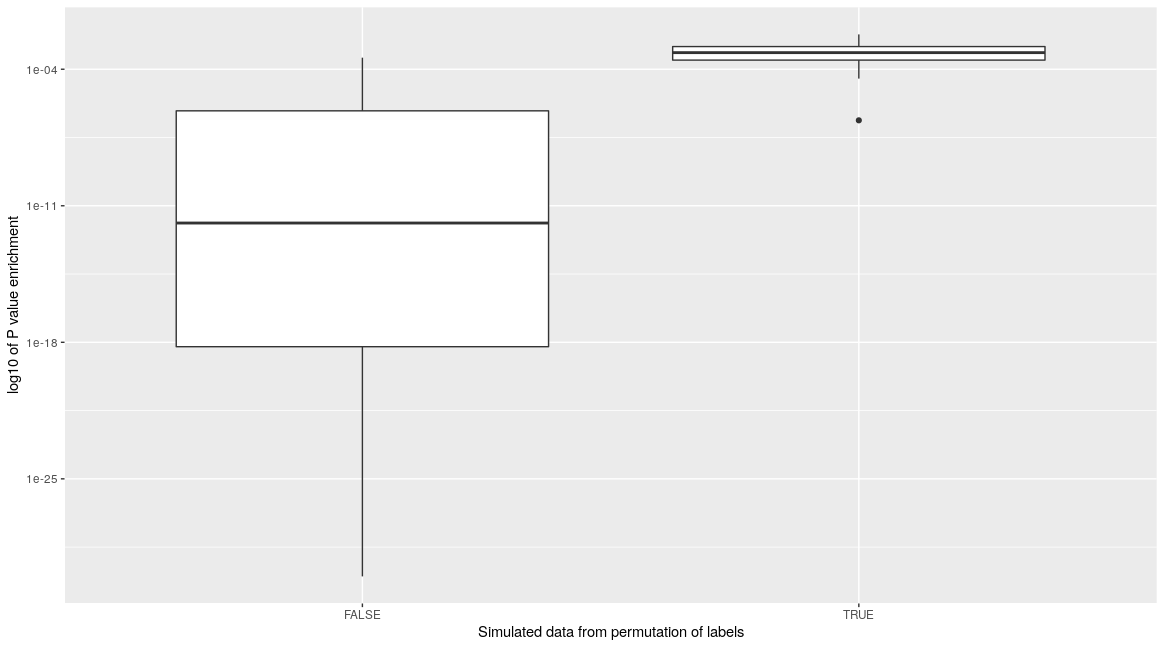
\includegraphics[width=0.9\textwidth]{images/Rplot_EnrichmentGO_permuted_labels.png}
    \caption{Enrichment p values for spectral groups Biological Process left compared with enrichment p values for groups of identical size derived from label permutation. Top p value for each group used.}
    \label{fig:topGO_permutation}
\end{figure}
% latex table generated in R 3.6.3 by xtable 1.8-4 package
% Sat Apr 11 15:28:29 2020
\begin{table}[ht]
\centering
\begin{adjustbox}{max width=\textwidth}
\begin{tabular}{lllrrrrl}
  \hline
community & GO.ID & Term & Annotated & Significant & Expected & classic & less\_than\_alpha \\ 
  \hline
1 & GO:0000226 & microtubule cytoskeleton organization & 201 & 44 & 9.64 & $3.20 \times 10^{-19}$ & TRUE \\ 
  2 & GO:0031145 & anaphase-promoting complex-dependent cat... & 34 & 30 & 1.64 & $1.00 \times 10^{-30}$ & TRUE \\ 
  3 & GO:0034762 & regulation of transmembrane transport & 203 & 10 & 2.25 & $4.60 \times 10^{-5}$ & FALSE \\ 
  4 & GO:0007031 & peroxisome organization & 36 & 13 & 0.33 & $4.30 \times 10^{-19}$ & TRUE \\ 
  5 & GO:0007186 & G protein-coupled receptor signaling pat... & 178 & 34 & 5.71 & $8.20 \times 10^{-19}$ & TRUE \\ 
  6 & GO:0097035 & regulation of membrane lipid distributio... & 9 & 5 & 0.19 & $4.50 \times 10^{-7}$ & TRUE \\ 
  7 & GO:0061640 & cytoskeleton-dependent cytokinesis & 50 & 11 & 1.84 & $1.20 \times 10^{-6}$ & TRUE \\ 
  9 & GO:0001894 & tissue homeostasis & 56 & 10 & 1.06 & $5.00 \times 10^{-8}$ & TRUE \\ 
  10 & GO:0042773 & ATP synthesis coupled electron transport & 56 & 43 & 2.57 & $1.00 \times 10^{-30}$ & TRUE \\ 
  11 & GO:0034498 & early endosome to Golgi transport & 5 & 3 & 0.08 & $3.70 \times 10^{-5}$ & FALSE \\ 
  12 & GO:0007041 & lysosomal transport & 51 & 14 & 0.50 & $3.70 \times 10^{-18}$ & TRUE \\ 
  16 & GO:0000045 & autophagosome assembly & 34 & 10 & 0.73 & $1.00 \times 10^{-9}$ & TRUE \\ 
  17 & GO:0061025 & membrane fusion & 70 & 28 & 2.92 & $9.40 \times 10^{-22}$ & TRUE \\ 
  19 & GO:0046755 & viral budding & 13 & 5 & 0.08 & $5.60 \times 10^{-9}$ & TRUE \\ 
  20 & GO:0006468 & protein phosphorylation & 535 & 65 & 23.57 & $9.70 \times 10^{-17}$ & TRUE \\ 
  22 & GO:0046328 & regulation of JNK cascade & 47 & 6 & 0.59 & $2.00 \times 10^{-5}$ & FALSE \\ 
  23 & GO:1900028 & negative regulation of ruffle assembly & 2 & 2 & 0.04 & $3.90 \times 10^{-4}$ & FALSE \\ 
  24 & GO:0006470 & protein dephosphorylation & 101 & 13 & 2.27 & $2.20 \times 10^{-7}$ & TRUE \\ 
  25 & GO:0072321 & chaperone-mediated protein transport & 7 & 3 & 0.06 & $1.60 \times 10^{-5}$ & FALSE \\ 
  26 & GO:0043408 & regulation of MAPK cascade & 172 & 33 & 6.08 & $7.40 \times 10^{-17}$ & TRUE \\ 
  28 & GO:1903361 & protein localization to basolateral plas... & 6 & 3 & 0.06 & $2.30 \times 10^{-5}$ & FALSE \\ 
  32 & GO:0051480 & regulation of cytosolic calcium ion conc... & 87 & 12 & 1.28 & $1.90 \times 10^{-9}$ & TRUE \\ 
  33 & GO:0006897 & endocytosis & 278 & 55 & 15.66 & $2.70 \times 10^{-18}$ & TRUE \\ 
  34 & GO:0007015 & actin filament organization & 172 & 60 & 10.62 & $1.00 \times 10^{-30}$ & TRUE \\ 
  43 & GO:0051276 & chromosome organization & 238 & 71 & 10.34 & $1.00 \times 10^{-30}$ & TRUE \\ 
  44 & GO:0006457 & protein folding & 102 & 25 & 3.06 & $2.60 \times 10^{-17}$ & TRUE \\ 
  45 & GO:0036503 & ERAD pathway & 27 & 13 & 0.98 & $1.30 \times 10^{-12}$ & TRUE \\ 
  46 & GO:0070202 & regulation of establishment of protein l... & 8 & 8 & 0.11 & $8.30 \times 10^{-16}$ & TRUE \\ 
  47 & GO:0035337 & fatty-acyl-CoA metabolic process & 19 & 3 & 0.15 & $3.70 \times 10^{-4}$ & FALSE \\ 
  48 & GO:0006183 & GTP biosynthetic process & 3 & 3 & 0.02 & $2.50 \times 10^{-7}$ & TRUE \\ 
  51 & GO:0006409 & tRNA export from nucleus & 12 & 9 & 0.40 & $6.70 \times 10^{-12}$ & TRUE \\ 
  53 & GO:0006413 & translational initiation & 120 & 106 & 14.17 & $1.00 \times 10^{-30}$ & TRUE \\ 
  55 & GO:0006397 & mRNA processing & 95 & 16 & 1.22 & $7.30 \times 10^{-15}$ & TRUE \\ 
  58 & GO:2001235 & positive regulation of apoptotic signali... & 53 & 6 & 0.59 & $1.90 \times 10^{-5}$ & FALSE \\ 
  62 & GO:0070125 & mitochondrial translational elongation & 32 & 15 & 0.32 & $1.00 \times 10^{-23}$ & TRUE \\ 
   \hline
\end{tabular}
\end{adjustbox}
\caption{Top term biological process Spectral clustering background PSP} 
\label{tab:Top term biological process spectral clustering background PSP}
\end{table}

% latex table generated in R 3.6.3 by xtable 1.8-4 package
% Sat Apr 11 15:39:02 2020
\begin{table}[ht]
\centering
\begin{adjustbox}{max width=\textwidth}
\begin{tabular}{lllrrrrl}
  \hline
community & GO.ID & Term & Annotated & Significant & Expected & classic & less\_than\_alpha \\ 
  \hline
1 & GO:0008017 & microtubule binding & 113 & 21 & 5.12 & $1.50 \times 10^{-8}$ & TRUE \\ 
  2 & GO:0004298 & threonine-type endopeptidase activity & 13 & 13 & 0.62 & $4.50 \times 10^{-18}$ & TRUE \\ 
  3 & GO:0008270 & zinc ion binding & 119 & 7 & 1.40 & $3.90 \times 10^{-4}$ & FALSE \\ 
  4 & GO:0031489 & myosin V binding & 14 & 4 & 0.13 & $5.90 \times 10^{-6}$ & TRUE \\ 
  5 & GO:0008066 & glutamate receptor activity & 21 & 12 & 0.66 & $1.10 \times 10^{-13}$ & TRUE \\ 
  6 & GO:0015247 & aminophospholipid transmembrane transpor... & 3 & 3 & 0.06 & $9.50 \times 10^{-6}$ & TRUE \\ 
  7 & GO:0005525 & GTP binding & 159 & 19 & 5.82 & $3.10 \times 10^{-6}$ & TRUE \\ 
  9 & GO:0005507 & copper ion binding & 12 & 4 & 0.23 & $5.30 \times 10^{-5}$ & FALSE \\ 
  10 & GO:0003954 & NADH dehydrogenase activity & 33 & 31 & 1.51 & $1.00 \times 10^{-30}$ & TRUE \\ 
  11 & GO:1990460 & leptin receptor binding & 3 & 3 & 0.05 & $3.90 \times 10^{-6}$ & TRUE \\ 
  12 & GO:0030674 & protein binding, bridging & 65 & 4 & 0.59 & $2.50 \times 10^{-3}$ & FALSE \\ 
  16 & GO:0005251 & delayed rectifier potassium channel acti... & 10 & 4 & 0.22 & $3.90 \times 10^{-5}$ & FALSE \\ 
  17 & GO:0000149 & SNARE binding & 61 & 37 & 2.64 & $1.00 \times 10^{-30}$ & TRUE \\ 
  19 & GO:0048306 & calcium-dependent protein binding & 32 & 3 & 0.19 & $8.40 \times 10^{-4}$ & FALSE \\ 
  20 & GO:0051018 & protein kinase A binding & 23 & 15 & 1.02 & $8.30 \times 10^{-16}$ & TRUE \\ 
  22 & GO:0004709 & MAP kinase kinase kinase activity & 11 & 3 & 0.14 & $2.90 \times 10^{-4}$ & FALSE \\ 
  23 & GO:0004115 & 3',5'-cyclic-AMP phosphodiesterase activ... & 4 & 2 & 0.07 & $2.00 \times 10^{-3}$ & FALSE \\ 
  24 & GO:0099181 & structural constituent of presynapse & 4 & 4 & 0.09 & $2.30 \times 10^{-7}$ & TRUE \\ 
  25 & GO:0005149 & interleukin-1 receptor binding & 2 & 2 & 0.02 & $5.50 \times 10^{-5}$ & FALSE \\ 
  26 & GO:0004708 & MAP kinase kinase activity & 9 & 8 & 0.32 & $1.60 \times 10^{-11}$ & TRUE \\ 
  28 & GO:0097016 & L27 domain binding & 4 & 4 & 0.04 & $1.30 \times 10^{-8}$ & TRUE \\ 
  32 & GO:0005261 & cation channel activity & 96 & 11 & 1.42 & $8.10 \times 10^{-8}$ & TRUE \\ 
  33 & GO:0017124 & SH3 domain binding & 55 & 29 & 3.08 & $5.60 \times 10^{-23}$ & TRUE \\ 
  34 & GO:0003779 & actin binding & 224 & 85 & 13.95 & $1.00 \times 10^{-30}$ & TRUE \\ 
  43 & GO:0003677 & DNA binding & 251 & 67 & 11.23 & $1.00 \times 10^{-30}$ & TRUE \\ 
  44 & GO:0031072 & heat shock protein binding & 52 & 25 & 1.54 & $6.30 \times 10^{-26}$ & TRUE \\ 
  45 & GO:0005342 & organic acid transmembrane transporter a... & 18 & 7 & 0.66 & $1.80 \times 10^{-6}$ & TRUE \\ 
  46 & GO:0051082 & unfolded protein binding & 56 & 9 & 0.78 & $4.00 \times 10^{-8}$ & TRUE \\ 
  47 & GO:0003996 & acyl-CoA ligase activity & 4 & 2 & 0.03 & $3.50 \times 10^{-4}$ & FALSE \\ 
  48 & GO:0061631 & ubiquitin conjugating enzyme activity & 8 & 3 & 0.05 & $1.40 \times 10^{-5}$ & TRUE \\ 
  51 & GO:0017056 & structural constituent of nuclear pore & 7 & 6 & 0.22 & $5.40 \times 10^{-9}$ & TRUE \\ 
  53 & GO:0003723 & RNA binding & 549 & 248 & 66.55 & $1.00 \times 10^{-30}$ & TRUE \\ 
  55 & GO:0003676 & nucleic acid binding & 716 & 24 & 9.09 & $5.00 \times 10^{-7}$ & TRUE \\ biological
  58 & GO:0048306 & calcium-dependent protein binding & 32 & 4 & 0.35 & $3.40 \times 10^{-4}$ & FALSE \\ 
  62 & GO:0003735 & structural constituent of ribosome & 101 & 11 & 0.95 & $6.30 \times 10^{-10}$ & TRUE \\ 
   \hline
\end{tabular}
\end{adjustbox}
\caption{Top term molecular function spectral clustering background PSP} 
\label{tab:Top term molecular function spectral clustering background PSP}
\end{table}



% latex table generated in R 3.6.3 by xtable 1.8-4 package
% Sat Apr 11 15:46:40 2020
\begin{table}[ht]
\centering
\begin{adjustbox}{max width=\textwidth}
\begin{tabular}{lllrrrrl}
  \hline
community & GO.ID & Term & Annotated & Significant & Expected & classic & less\_than\_alpha \\ 
  \hline
1 & GO:0005815 & microtubule organizing center & 238 & 57 & 11.51 & $3.20 \times 10^{-27}$ & TRUE \\ 
  2 & GO:0000502 & proteasome complex & 37 & 34 & 1.78 & $1.00 \times 10^{-30}$ & TRUE \\ 
  3 & GO:0016010 & dystrophin-associated glycoprotein compl... & 8 & 5 & 0.09 & $9.60 \times 10^{-9}$ & TRUE \\ 
  4 & GO:0005777 & peroxisome & 61 & 14 & 0.56 & $1.60 \times 10^{-17}$ & TRUE \\ 
  5 & GO:0005834 & heterotrimeric G-protein complex & 18 & 12 & 0.59 & $1.30 \times 10^{-14}$ & TRUE \\ 
  6 & GO:0016021 & integral component of membrane & 747 & 32 & 16.52 & $4.20 \times 10^{-5}$ & FALSE \\ 
   7 & GO:0005940 & septin ring & 11 & 11 & 0.40 & $1.00 \times 10^{-16}$ & TRUE \\ 
  9 & GO:0072562 & blood microparticle & 52 & 9 & 1.00 & $3.80 \times 10^{-7}$ & TRUE \\ 
  10 & GO:0070469 & respiratory chain & 54 & 42 & 2.44 & $1.00 \times 10^{-30}$ & TRUE \\ 
  11 & GO:0030905 & retromer, tubulation complex & 4 & 4 & 0.07 & $6.70 \times 10^{-8}$ & TRUE \\ 
  12 & GO:0030897 & HOPS complex & 7 & 7 & 0.07 & $5.30 \times 10^{-15}$ & TRUE \\ 
  16 & GO:0000421 & autophagosome membrane & 11 & 6 & 0.23 & $3.20 \times 10^{-8}$ & TRUE \\ 
  17 & GO:0031201 & SNARE complex & 28 & 25 & 1.18 & $1.00 \times 10^{-30}$ & TRUE \\ 
  19 & GO:0000813 & ESCRT I complex & 3 & 3 & 0.02 & $1.50 \times 10^{-7}$ & TRUE \\ 
  20 & GO:0005886 & plasma membrane & 1276 & 94 & 56.07 & $1.10 \times 10^{-10}$ & TRUE \\ 
  22 & GO:0008043 & intracellular ferritin complex & 2 & 2 & 0.02 & $1.50 \times 10^{-4}$ & FALSE \\ 
  23 & GO:0034045 & phagophore assembly site membrane & 8 & 2 & 0.16 & $9.70 \times 10^{-3}$ & FALSE \\ 
  24 & GO:0000159 & protein phosphatase type 2A complex & 10 & 7 & 0.22 & $2.20 \times 10^{-10}$ & TRUE \\ 
  25 & GO:0042719 & mitochondrial intermembrane space protei... & 3 & 2 & 0.02 & $1.70 \times 10^{-4}$ & FALSE \\ 
  26 & GO:0071944 & cell periphery & 1338 & 78 & 47.35 & $7.70 \times 10^{-9}$ & TRUE \\ 
  28 & GO:0005923 & bicellular tight junction & 44 & 11 & 0.47 & $2.20 \times 10^{-13}$ & TRUE \\ 
  32 & GO:0034703 & cation channel complex & 96 & 11 & 1.47 & $1.20 \times 10^{-7}$ & TRUE \\ 
  33 & GO:0071944 & cell periphery & 1338 & 121 & 74.18 & $1.10 \times 10^{-12}$ & TRUE \\ 
  34 & GO:0015629 & actin cytoskeleton & 260 & 92 & 16.25 & $1.00 \times 10^{-30}$ & TRUE \\ 
  43 & GO:0031981 & nuclear lumen & 856 & 111 & 36.86 & $1.00 \times 10^{-30}$ & TRUE \\ 
  44 & GO:0101031 & chaperone complex & 20 & 8 & 0.59 & $4.10 \times 10^{-8}$ & TRUE \\ 
  45 & GO:0044432 & endoplasmic reticulum part & 292 & 32 & 10.68 & $5.40 \times 10^{-9}$ & TRUE \\ 
  46 & GO:0005832 & chaperonin-containing T-complex & 9 & 9 & 0.13 & $1.00 \times 10^{-17}$ & TRUE \\ 
  47 & GO:0005778 & peroxisomal membrane & 33 & 5 & 0.25 & $3.60 \times 10^{-6}$ & TRUE \\ 
  48 & GO:0031371 & ubiquitin conjugating enzyme complex & 5 & 3 & 0.03 & $2.00 \times 10^{-6}$ & TRUE \\ 
  51 & GO:0005643 & nuclear pore & 25 & 12 & 0.81 & $2.70 \times 10^{-12}$ & TRUE \\ 
  53 & GO:1990904 & ribonucleoprotein complex & 293 & 184 & 34.65 & $1.00 \times 10^{-30}$ & TRUE \\ 
  55 & GO:0016607 & nuclear speck & 83 & 15 & 1.08 & $2.40 \times 10^{-14}$ & TRUE \\ 
  58 & GO:0030127 & COPII vesicle coat & 9 & 4 & 0.10 & $1.50 \times 10^{-6}$ & TRUE \\ 
  62 & GO:0000315 & organellar large ribosomal subunit & 15 & 14 & 0.15 & $7.00 \times 10^{-29}$ & TRUE \\ 
   \hline
\end{tabular}
\end{adjustbox}
\caption{Top term CC background spectral clustering PSP} 
\label{tab:Top term CC background spectral clustering PSP}
\end{table}

\begin{table}[]
    \centering
    \begin{tabular}{lllll}
    \toprule
          & Degree & Eigenvector centrality & Closeness & Betweenness \\
         \midrule
    Degree  & 1  & 0.92  & 0.66 & 0.85\\
    Eigenvector centrality & 0.92 & 1 & 0.63 & 0.72  \\
    Closeness & 0.66 & 0.63 & 1 & 0.44  \\
    Betweenness& 0.85 & 0.72 & 0.44 & 1 \\
    \bottomrule
    \end{tabular}
    \caption{Correlation of centrality measures for 58 sociometric network datasets from Valente et al \cite{valente2008correlated}. Pearson correlation coefficient. Values are for symmetrised closeness and betweenness centrality. Eigenvector centrality is necessarily symmetrised. Range of average network size 45-83. Some studies had maximal nominations for degree}
    \label{tab:Correlation of centrality valente et al}
\end{table}

\subsection{GO Louvain}
% latex table generated in R 3.6.3 by xtable 1.8-4 package
% Sat Apr 18 17:57:38 2020
\begin{table}[ht]
\centering
\begin{adjustbox}{max width=\textwidth}
\begin{tabular}{lllrrrrl}
  \hline
community & GO.ID & Term & Annotated & Significant & Expected & classic & less\_than\_alpha \\ 
  \hline
1 & GO:0006625 & protein targeting to peroxisome & 29 & 16 & 2 & $5.70 \times 10^{-13}$ & TRUE \\ 
  2 & GO:0042773 & ATP synthesis coupled electron transport & 56 & 45 & 6 & $1.00 \times 10^{-30}$ & TRUE \\ 
  3 & GO:0016071 & mRNA metabolic process & 254 & 165 & 39 & $1.00 \times 10^{-30}$ & TRUE \\ 
  4 & GO:0051276 & chromosome organization & 238 & 99 & 18 & $1.00 \times 10^{-30}$ & TRUE \\ 
  5 & GO:0070202 & regulation of establishment of protein l... & 8 & 8 & 0 & $1.00 \times 10^{-12}$ & TRUE \\ 
  6 & GO:0031145 & anaphase-promoting complex-dependent cat... & 34 & 30 & 2 & $1.00 \times 10^{-30}$ & TRUE \\ 
  7 & GO:0007215 & glutamate receptor signaling pathway & 64 & 25 & 3 & $1.30 \times 10^{-18}$ & TRUE \\ 
  8 & GO:0006468 & protein phosphorylation & 535 & 196 & 84 & $1.00 \times 10^{-30}$ & TRUE \\ 
  9 & GO:0030029 & actin filament-based process & 333 & 141 & 43 & $1.00 \times 10^{-30}$ & TRUE \\ 
  10 & GO:0016236 & macroautophagy & 125 & 19 & 2 & $5.60 \times 10^{-14}$ & TRUE \\ 
  11 & GO:0097711 & ciliary basal body-plasma membrane docki... & 48 & 27 & 5 & $4.70 \times 10^{-16}$ & TRUE \\ 
  12 & GO:0015696 & ammonium transport & 25 & 4 & 0 & $1.30 \times 10^{-5}$ & FALSE \\ 
  13 & GO:0001732 & formation of cytoplasmic translation ini... & 11 & 10 & 0 & $3.30 \times 10^{-16}$ & TRUE \\ 
  14 & GO:0061025 & membrane fusion & 70 & 30 & 4 & $1.30 \times 10^{-21}$ & TRUE \\ 
   \hline
\end{tabular}
\end{adjustbox}
\caption{Top term  lourvain BP background PSP} 
\label{tab:Top term  lourvain BP background PSP}
\end{table}

% latex table generated in R 3.6.3 by xtable 1.8-4 package
% Sat Apr 18 17:58:35 2020
\begin{table}[ht]
\centering
\begin{tabular}{lr}
  \hline
quantile & value of p \\ 
  \hline
0\% & $1.000 \times 10^{-30}$ \\ 
  25\% & $1.000 \times 10^{-30}$ \\ 
  50\% & $6.506 \times 10^{-19}$ \\ 
  75\% & $4.212 \times 10^{-14}$ \\ 
  100\% & $1.300 \times 10^{-5}$ \\ 
   \hline
\end{tabular}
\caption{P values for different quantiles for lourvain clusteringBP} 
\label{tabP values for different quantiles for lourvain clusteringBP}
\end{table}

\subsubsection{Molecular function}
% latex table generated in R 3.6.3 by xtable 1.8-4 package
% Sat Apr 18 17:59:47 2020
\begin{table}[ht]
\centering
\begin{adjustbox}{max width=\textwidth}
\begin{tabular}{lllrrrrl}
  \hline
community & GO.ID & Term & Annotated & Significant & Expected & classic & less\_than\_alpha \\ 
  \hline
1 & GO:0034987 & immunoglobulin receptor binding & 8 & 6 & 0 & $1.10 \times 10^{-6}$ & TRUE \\ 
  2 & GO:0003954 & NADH dehydrogenase activity & 33 & 30 & 3 & $1.60 \times 10^{-27}$ & TRUE \\ 
  3 & GO:0003723 & RNA binding & 549 & 298 & 86 & $1.00 \times 10^{-30}$ & TRUE \\ 
  4 & GO:0003677 & DNA binding & 251 & 86 & 20 & $1.00 \times 10^{-30}$ & TRUE \\ 
  5 & GO:0051721 & protein phosphatase 2A binding & 9 & 6 & 0 & $9.10 \times 10^{-8}$ & TRUE \\ 
  6 & GO:0004298 & threonine-type endopeptidase activity & 13 & 13 & 1 & $4.90 \times 10^{-18}$ & TRUE \\ 
  7 & GO:0038023 & signaling receptor activity & 128 & 32 & 6 & $5.40 \times 10^{-17}$ & TRUE \\ 
  8 & GO:0004672 & protein kinase activity & 195 & 103 & 30 & $1.00 \times 10^{-30}$ & TRUE \\ 
  9 & GO:0003779 & actin binding & 224 & 107 & 29 & $1.00 \times 10^{-30}$ & TRUE \\ 
  10 & GO:0017137 & Rab GTPase binding & 63 & 10 & 1 & $6.50 \times 10^{-8}$ & TRUE \\ 
  11 & GO:0008017 & microtubule binding & 113 & 30 & 11 & $1.40 \times 10^{-7}$ & TRUE \\ 
  12 & GO:0005544 & calcium-dependent phospholipid binding & 27 & 4 & 0 & $1.90 \times 10^{-5}$ & TRUE \\ 
  13 & GO:0003743 & translation initiation factor activity & 27 & 14 & 1 & $5.20 \times 10^{-17}$ & TRUE \\ 
  14 & GO:0000149 & SNARE binding & 61 & 33 & 3 & $1.70 \times 10^{-28}$ & TRUE \\ 
   \hline
\end{tabular}
\end{adjustbox}
\caption{Top term  lourvain MF background PSP} 
\label{tab:Top term  lourvain MF background PSP}
\end{table}


% latex table generated in R 3.6.3 by xtable 1.8-4 package
% Sat Apr 18 18:00:33 2020
\begin{table}[ht]
\centering

\begin{tabular}{lr}
  \hline
quantile & value of p \\ 
  \hline
0\% & $1.000 \times 10^{-30}$ \\ 
  25\% & $4.325 \times 10^{-29}$ \\ 
  50\% & $2.845 \times 10^{-17}$ \\ 
  75\% & $8.450 \times 10^{-8}$ \\ 
  100\% & $1.900 \times 10^{-5}$ \\ 
   \hline
\end{tabular}
\caption{P values for different quantiles for lourvain clusteringMF} 
\label{tabP values for different quantiles for lourvain clusteringMF}
\end{table}

\subsubsection{Cellular compartment}



\subsection{topgo Infomap}

% latex table generated in R 3.6.3 by xtable 1.8-4 package
% Sat Apr 18 18:17:43 2020
% latex table generated in R 3.6.3 by xtable 1.8-4 package
% Sat Apr 18 18:35:49 2020
\begin{table}[ht]
\centering
\begin{adjustbox}{max width=\textwidth}
\begin{tabular}{lllrrrrl}
  \hline
community & GO.ID & Term & Annotated & Significant & Expected & classic & less\_than\_alpha \\ 
  \hline
1 & GO:0090304 & nucleic acid metabolic process & 801 & 505 & 287 & $1.00 \times 10^{-30}$ & TRUE \\ 
  2 & GO:0030029 & actin filament-based process & 333 & 71 & 12 & $1.00 \times 10^{-30}$ & TRUE \\ 
  3 & GO:0006897 & endocytosis & 278 & 41 & 10 & $2.60 \times 10^{-17}$ & TRUE \\ 
  4 & GO:0000226 & microtubule cytoskeleton organization & 201 & 28 & 5 & $2.90 \times 10^{-16}$ & TRUE \\ 
  5 & GO:0070202 & regulation of establishment of protein l... & 8 & 8 & 0 & $1.20 \times 10^{-15}$ & TRUE \\ 
  6 & GO:0006521 & regulation of cellular amino acid metabo... & 33 & 28 & 0 & $1.00 \times 10^{-30}$ & TRUE \\ 
  7 & GO:0070268 & cornification & 41 & 12 & 1 & $9.90 \times 10^{-13}$ & TRUE \\ 
  8 & GO:0045821 & positive regulation of glycolytic proces... & 5 & 2 & 0 & $3.30 \times 10^{-3}$ & FALSE \\ 
  9 & GO:0090383 & phagosome acidification & 15 & 15 & 0 & $4.30 \times 10^{-29}$ & TRUE \\ 
  10 & GO:0030036 & actin cytoskeleton organization & 284 & 28 & 4 & $5.00 \times 10^{-18}$ & TRUE \\ 
  11 & GO:0099537 & trans-synaptic signaling & 316 & 28 & 5 & $1.80 \times 10^{-16}$ & TRUE \\ 
  12 & GO:0010257 & NADH dehydrogenase complex assembly & 34 & 31 & 0 & $1.00 \times 10^{-30}$ & TRUE \\ 
  13 & GO:0060384 & innervation & 10 & 2 & 0 & $5.10 \times 10^{-3}$ & FALSE \\ 
  14 & GO:0061025 & membrane fusion & 70 & 25 & 1 & $1.00 \times 10^{-30}$ & TRUE \\ 
  15 & GO:0000045 & autophagosome assembly & 34 & 10 & 0 & $2.20 \times 10^{-13}$ & TRUE \\ 
  16 & GO:0007186 & G protein-coupled receptor signaling pat... & 178 & 25 & 2 & $2.70 \times 10^{-26}$ & TRUE \\ 
  17 & GO:0034199 & activation of protein kinase A activity & 10 & 6 & 0 & $1.10 \times 10^{-11}$ & TRUE \\ 
  18 & GO:0010921 & regulation of phosphatase activity & 56 & 10 & 1 & $2.60 \times 10^{-11}$ & TRUE \\ 
  19 & GO:0005513 & detection of calcium ion & 5 & 3 & 0 & $4.20 \times 10^{-6}$ & TRUE \\ 
  20 & GO:0070125 & mitochondrial translational elongation & 32 & 16 & 0 & $6.80 \times 10^{-28}$ & TRUE \\ 
  21 & GO:0031175 & neuron projection development & 404 & 10 & 3 & $1.60 \times 10^{-4}$ & FALSE \\ 
  22 & GO:0006893 & Golgi to plasma membrane transport & 33 & 5 & 0 & $3.90 \times 10^{-6}$ & TRUE \\ 
  23 & GO:0002495 & antigen processing and presentation of p... & 53 & 10 & 0 & $6.90 \times 10^{-14}$ & TRUE \\ 
  24 & GO:0007215 & glutamate receptor signaling pathway & 64 & 13 & 0 & $5.80 \times 10^{-18}$ & TRUE \\ 
  25 & GO:0051403 & stress-activated MAPK cascade & 80 & 12 & 0 & $8.70 \times 10^{-17}$ & TRUE \\ 
  27 & GO:0006869 & lipid transport & 65 & 5 & 0 & $1.20 \times 10^{-5}$ & FALSE \\ 
  28 & GO:0002221 & pattern recognition receptor signaling p... & 40 & 5 & 0 & $1.10 \times 10^{-6}$ & TRUE \\ 
  29 & GO:0006816 & calcium ion transport & 144 & 14 & 1 & $1.10 \times 10^{-16}$ & TRUE \\ 
  30 & GO:0006637 & acyl-CoA metabolic process & 40 & 10 & 0 & $3.30 \times 10^{-16}$ & TRUE \\ 
  31 & GO:1902531 & regulation of intracellular signal trans... & 468 & 7 & 2 & $2.40 \times 10^{-3}$ & FALSE \\ 
  32 & GO:0061640 & cytoskeleton-dependent cytokinesis & 50 & 11 & 0 & $3.50 \times 10^{-18}$ & TRUE \\ 
  34 & GO:0006625 & protein targeting to peroxisome & 29 & 14 & 0 & $9.80 \times 10^{-28}$ & TRUE \\ 
  35 & GO:1904340 & positive regulation of dopaminergic neur... & 2 & 2 & 0 & $1.60 \times 10^{-5}$ & FALSE \\ 
  36 & GO:0006957 & complement activation, alternative pathw... & 2 & 2 & 0 & $2.70 \times 10^{-5}$ & FALSE \\ 
  40 & GO:0006936 & muscle contraction & 124 & 7 & 1 & $2.30 \times 10^{-7}$ & TRUE \\ 
  46 & GO:0034204 & lipid translocation & 6 & 4 & 0 & $3.90 \times 10^{-9}$ & TRUE \\ 
  52 & GO:0098659 & inorganic cation import across plasma me... & 25 & 4 & 0 & $2.30 \times 10^{-6}$ & TRUE \\ 
   \hline
\end{tabular}
\end{adjustbox}
\caption{Top term  infomap BP background PSP} 
\label{tab:Top term  infomap BP background PSP}
\end{table}


% latex table generated in R 3.6.3 by xtable 1.8-4 package
% Sat Apr 18 18:17:43 2020
\begin{table}[ht]
\centering

\begin{tabular}{lr}
  \hline
quantile & value of p \\ 
  \hline
0\% & $1.000 \times 10^{-30}$ \\ 
  25\% & $3.500 \times 10^{-18}$ \\ 
  50\% & $1.200 \times 10^{-15}$ \\ 
  75\% & $2.300 \times 10^{-6}$ \\ 
  100\% & $5.100 \times 10^{-3}$ \\ 
   \hline
\end{tabular}
\caption{P values for different quantiles for infomap clusteringBP} 
\label{tabP values for different quantiles for infomap clusteringBP}
\end{table}

\subsubsection{MF topgo infomap}
% latex table generated in R 3.6.3 by xtable 1.8-4 package
% Sat Apr 18 20:16:53 2020
\begin{table}[ht]
\centering
\begin{adjustbox}{max width=\textwidth}
\begin{tabular}{lllrrrrl}
  \hline
community & GO.ID & Term & Annotated & Significant & Expected & classic & less\_than\_alpha \\ 
  \hline
1 & GO:1990904 & ribonucleoprotein complex & 293 & 230 & 105 & $1.00 \times 10^{-30}$ & TRUE \\ 
  2 & GO:0015629 & actin cytoskeleton & 260 & 79 & 10 & $1.00 \times 10^{-30}$ & TRUE \\ 
  3 & GO:0071944 & cell periphery & 1338 & 91 & 46 & $9.40 \times 10^{-18}$ & TRUE \\ 
  4 & GO:0015630 & microtubule cytoskeleton & 407 & 48 & 9 & $1.40 \times 10^{-25}$ & TRUE \\ 
  5 & GO:0005832 & chaperonin-containing T-complex & 9 & 9 & 0 & $1.50 \times 10^{-17}$ & TRUE \\ 
  6 & GO:0000502 & proteasome complex & 37 & 31 & 0 & $1.00 \times 10^{-30}$ & TRUE \\ 
  7 & GO:0005882 & intermediate filament & 64 & 13 & 1 & $4.40 \times 10^{-11}$ & TRUE \\ 
  8 & GO:0097427 & microtubule bundle & 5 & 2 & 0 & $3.40 \times 10^{-3}$ & FALSE \\ 
  9 & GO:0033176 & proton-transporting V-type ATPase comple... & 13 & 13 & 0 & $2.10 \times 10^{-25}$ & TRUE \\ 
  10 & GO:0031209 & SCAR complex & 8 & 7 & 0 & $5.70 \times 10^{-13}$ & TRUE \\ 
  11 & GO:0097060 & synaptic membrane & 219 & 29 & 3 & $2.30 \times 10^{-22}$ & TRUE \\ 
  12 & GO:0005747 & mitochondrial respiratory chain complex ... & 34 & 31 & 0 & $1.00 \times 10^{-30}$ & TRUE \\ 
  13 & GO:0031232 & extrinsic component of external side of ... & 4 & 1 & 0 & $4.60 \times 10^{-2}$ & FALSE \\ 
  14 & GO:0031201 & SNARE complex & 28 & 25 & 0 & $1.00 \times 10^{-30}$ & TRUE \\ 
  15 & GO:0000421 & autophagosome membrane & 11 & 7 & 0 & $1.30 \times 10^{-12}$ & TRUE \\ 
  16 & GO:0005834 & heterotrimeric G-protein complex & 18 & 11 & 0 & $5.20 \times 10^{-19}$ & TRUE \\ 
  17 & GO:0005952 & cAMP-dependent protein kinase complex & 8 & 7 & 0 & $1.90 \times 10^{-15}$ & TRUE \\ 
  18 & GO:0000164 & protein phosphatase type 1 complex & 5 & 3 & 0 & $6.80 \times 10^{-6}$ & TRUE \\ 
  19 & GO:0034704 & calcium channel complex & 33 & 5 & 0 & $4.40 \times 10^{-6}$ & TRUE \\ 
  20 & GO:0000315 & organellar large ribosomal subunit & 15 & 15 & 0 & $1.00 \times 10^{-30}$ & TRUE \\ 
  21 & GO:0048787 & presynaptic active zone membrane & 18 & 2 & 0 & $5.80 \times 10^{-3}$ & FALSE \\ 
  22 & GO:0099023 & tethering complex & 33 & 5 & 0 & $3.60 \times 10^{-6}$ & TRUE \\ 
  23 & GO:0005875 & microtubule associated complex & 57 & 13 & 0 & $1.40 \times 10^{-19}$ & TRUE \\ 
  24 & GO:0045211 & postsynaptic membrane & 160 & 16 & 1 & $1.70 \times 10^{-17}$ & TRUE \\ 
  25 & GO:0097458 & neuron part & 812 & 10 & 4 & $2.10 \times 10^{-3}$ & FALSE \\ 
  27 & GO:0030905 & retromer, tubulation complex & 4 & 4 & 0 & $4.30 \times 10^{-10}$ & TRUE \\ 
  28 & GO:0005741 & mitochondrial outer membrane & 86 & 5 & 0 & $4.50 \times 10^{-5}$ & FALSE \\ 
  29 & GO:0016529 & sarcoplasmic reticulum & 31 & 8 & 0 & $7.60 \times 10^{-13}$ & TRUE \\ 
  30 & GO:0045254 & pyruvate dehydrogenase complex & 6 & 6 & 0 & $5.90 \times 10^{-15}$ & TRUE \\ 
  31 & GO:0038038 & G protein-coupled receptor homodimeric c... & 1 & 1 & 0 & $4.40 \times 10^{-3}$ & FALSE \\ 
  32 & GO:0005940 & septin ring & 11 & 11 & 0 & $8.10 \times 10^{-29}$ & TRUE \\ 
  34 & GO:0005777 & peroxisome & 61 & 17 & 0 & $3.40 \times 10^{-30}$ & TRUE \\ 
  35 & GO:0030285 & integral component of synaptic vesicle m... & 19 & 2 & 0 & $2.60 \times 10^{-3}$ & FALSE \\ 
  36 & GO:0072562 & blood microparticle & 52 & 7 & 0 & $3.70 \times 10^{-9}$ & TRUE \\ 
  40 & GO:0016010 & dystrophin-associated glycoprotein compl... & 8 & 5 & 0 & $4.50 \times 10^{-11}$ & TRUE \\ 
  46 & GO:0016021 & integral component of membrane & 747 & 12 & 3 & $2.80 \times 10^{-6}$ & TRUE \\ 
  52 & GO:0016021 & integral component of membrane & 747 & 13 & 3 & $1.80 \times 10^{-7}$ & TRUE \\ 
   \hline
\end{tabular}
\end{adjustbox}


\caption{Top term  infomap CC background PSP} 
\label{tab:Top term  infomap CC background PSP}
\end{table}
% latex table generated in R 3.6.3 by xtable 1.8-4 package
% Sat Apr 18 20:16:53 2020
\begin{table}[ht]
\centering
\begin{tabular}{lr}
  \hline
quantile & value of p \\ 
  \hline
0\% & $1.000 \times 10^{-30}$ \\ 
  25\% & $2.100 \times 10^{-25}$ \\ 
  50\% & $5.700 \times 10^{-13}$ \\ 
  75\% & $3.600 \times 10^{-6}$ \\ 
  100\% & $4.600 \times 10^{-2}$ \\ 
   \hline
\end{tabular}
\caption{P values for different quantiles for infomap clusteringCC} 
\label{tabP values for different quantiles for infomap clusteringCC}
\end{table}


% latex table generated in R 3.6.3 by xtable 1.8-4 package
% Sat Apr 18 18:37:55 2020
\begin{table}[ht]
\centering
\begin{adjustbox}{max width=\textwidth}
\begin{tabular}{lllrrrrl}
  \hline
community & GO.ID & Term & Annotated & Significant & Expected & classic & less\_than\_alpha \\ 
  \hline
1 & GO:0003676 & nucleic acid binding & 716 & 506 & 260 & $1.00 \times 10^{-30}$ & TRUE \\ 
  2 & GO:0003779 & actin binding & 224 & 76 & 9 & $1.00 \times 10^{-30}$ & TRUE \\ 
  3 & GO:0017124 & SH3 domain binding & 55 & 22 & 2 & $2.90 \times 10^{-19}$ & TRUE \\ 
  4 & GO:0008017 & microtubule binding & 113 & 11 & 2 & $1.80 \times 10^{-5}$ & TRUE \\ 
  5 & GO:0019888 & protein phosphatase regulator activity & 24 & 7 & 0 & $2.90 \times 10^{-8}$ & TRUE \\ 
  6 & GO:0004298 & threonine-type endopeptidase activity & 13 & 12 & 0 & $2.90 \times 10^{-23}$ & TRUE \\ 
  7 & GO:0005200 & structural constituent of cytoskeleton & 74 & 6 & 1 & $2.30 \times 10^{-3}$ & FALSE \\ 
  8 & GO:0016836 & hydro-lyase activity & 22 & 5 & 0 & $3.20 \times 10^{-5}$ & FALSE \\ 
  9 & GO:0036442 & proton-exporting ATPase activity & 19 & 14 & 0 & $4.90 \times 10^{-23}$ & TRUE \\ 
  10 & GO:0017048 & Rho GTPase binding & 79 & 16 & 1 & $2.90 \times 10^{-15}$ & TRUE \\ 
  11 & GO:0030165 & PDZ domain binding & 41 & 10 & 1 & $1.90 \times 10^{-10}$ & TRUE \\ 
  12 & GO:0003954 & NADH dehydrogenase activity & 33 & 30 & 0 & $1.00 \times 10^{-30}$ & TRUE \\ 
  13 & GO:0004860 & protein kinase inhibitor activity & 20 & 3 & 0 & $1.40 \times 10^{-3}$ & FALSE \\ 
  14 & GO:0000149 & SNARE binding & 61 & 29 & 1 & $1.00 \times 10^{-30}$ & TRUE \\ 
  15 & GO:0017137 & Rab GTPase binding & 63 & 9 & 1 & $6.60 \times 10^{-9}$ & TRUE \\ 
  16 & GO:0003924 & GTPase activity & 153 & 21 & 1 & $2.00 \times 10^{-21}$ & TRUE \\ 
  17 & GO:0051018 & protein kinase A binding & 23 & 11 & 0 & $3.60 \times 10^{-20}$ & TRUE \\ 
  18 & GO:0019888 & protein phosphatase regulator activity & 24 & 7 & 0 & $5.70 \times 10^{-10}$ & TRUE \\ 
  19 & GO:0005516 & calmodulin binding & 103 & 8 & 1 & $3.30 \times 10^{-7}$ & TRUE \\ 
  20 & GO:0003735 & structural constituent of ribosome & 101 & 12 & 1 & $2.30 \times 10^{-12}$ & TRUE \\ 
  21 & GO:0031005 & filamin binding & 5 & 3 & 0 & $2.90 \times 10^{-6}$ & TRUE \\ 
  22 & GO:0004823 & leucine-tRNA ligase activity & 1 & 1 & 0 & $7.60 \times 10^{-3}$ & FALSE \\ 
  23 & GO:0003774 & motor activity & 67 & 6 & 0 & $1.70 \times 10^{-6}$ & TRUE \\ 
  24 & GO:0008066 & glutamate receptor activity & 21 & 12 & 0 & $1.00 \times 10^{-23}$ & TRUE \\ 
  25 & GO:0004712 & protein serine/threonine/tyrosine kinase... & 15 & 5 & 0 & $5.50 \times 10^{-9}$ & TRUE \\ 
  27 & GO:1990460 & leptin receptor binding & 3 & 3 & 0 & $1.40 \times 10^{-7}$ & TRUE \\ 
  28 & GO:0019900 & kinase binding & 250 & 6 & 1 & $1.10 \times 10^{-3}$ & FALSE \\ 
  29 & GO:0005262 & calcium channel activity & 47 & 9 & 0 & $4.70 \times 10^{-13}$ & TRUE \\ 
  30 & GO:0016903 & oxidoreductase activity, acting on the a... & 21 & 8 & 0 & $1.40 \times 10^{-14}$ & TRUE \\ 
  31 & GO:0017048 & Rho GTPase binding & 79 & 3 & 0 & $3.90 \times 10^{-3}$ & FALSE \\ 
  32 & GO:0003924 & GTPase activity & 153 & 11 & 1 & $1.70 \times 10^{-12}$ & TRUE \\ 
  34 & GO:0071949 & FAD binding & 9 & 3 & 0 & $1.10 \times 10^{-5}$ & TRUE \\ 
  35 & GO:0050321 & tau-protein kinase activity & 17 & 2 & 0 & $1.90 \times 10^{-3}$ & FALSE \\ 
  36 & GO:0019825 & oxygen binding & 4 & 2 & 0 & $1.70 \times 10^{-4}$ & FALSE \\ 
  40 & GO:0008270 & zinc ion binding & 119 & 6 & 1 & $7.30 \times 10^{-6}$ & TRUE \\ 
  46 & GO:0015247 & aminophospholipid transmembrane transpor... & 3 & 3 & 0 & $6.00 \times 10^{-8}$ & TRUE \\ 
  52 & GO:0022857 & transmembrane transporter activity & 250 & 8 & 1 & $1.90 \times 10^{-6}$ & TRUE \\ 
   \hline
\end{tabular}
\end{adjustbox}
\caption{Top term  infomap MF background PSP} 
\label{tab:Top term  infomap MF background PSP}
\end{table}
% latex table generated in R 3.6.3 by xtable 1.8-4 package
% Sat Apr 18 18:37:55 2020
\begin{table}[ht]
\centering
\begin{tabular}{lr}
  \hline
quantile & value of p \\ 
  \hline
0\% & $1.000 \times 10^{-30}$ \\ 
  25\% & $2.900 \times 10^{-19}$ \\ 
  50\% & $6.600 \times 10^{-9}$ \\ 
  75\% & $1.100 \times 10^{-5}$ \\ 
  100\% & $7.600 \times 10^{-3}$ \\ 
   \hline
\end{tabular}
\caption{P values for different quantiles for infomap clusteringMF} 
\label{tabP values for different quantiles for infomap clusteringMF}
\end{table}

\subsection{lec}

% latex table generated in R 3.6.3 by xtable 1.8-4 package
% Sat Apr 18 20:20:18 2020
\begin{table}[ht]
\centering
\begin{adjustbox}{max width=\textwidth}
\begin{tabular}{lllrrrrl}
  \hline
community & GO.ID & Term & Annotated & Significant & Expected & classic & less\_than\_alpha \\ 
  \hline
1 & GO:0030036 & actin cytoskeleton organization & 284 & 188 & 94 & $1.00 \times 10^{-30}$ & TRUE \\ 
  2 & GO:0034641 & cellular nitrogen compound metabolic pro... & 1208 & 621 & 394 & $1.00 \times 10^{-30}$ & TRUE \\ 
  3 & GO:0010257 & NADH dehydrogenase complex assembly & 34 & 33 & 12 & $8.10 \times 10^{-15}$ & TRUE \\ 
   \hline
\end{tabular}
\end{adjustbox}
\caption{Top term  lec BP background PSP} 
\label{tab:Top term  lec BP background PSP}
\end{table}

% latex table generated in R 3.6.3 by xtable 1.8-4 package
% Sat Apr 18 20:20:18 2020
\begin{table}[ht]
\centering
\begin{tabular}{lr}
  \hline
quantile & value of p \\ 
  \hline
0\% & $1.000 \times 10^{-30}$ \\ 
  25\% & $1.000 \times 10^{-30}$ \\ 
  50\% & $1.000 \times 10^{-30}$ \\ 
  75\% & $4.050 \times 10^{-15}$ \\ 
  100\% & $8.100 \times 10^{-15}$ \\ 
   \hline
\end{tabular}
\caption{P values for different quantiles for lec clusteringBP} 
\label{tabP values for different quantiles for lec clusteringBP}
\end{table}

\subsection{Lec size off}

greater than 5

\section{Ontology of centrality measures}
code for eigenvector at \url{source('~/RProjects/group_sizes/R/plotting/modified_exampleGoObject_summary_PSP_centrality_eigenvector.R')}
\subsection{Betweenness}
% latex table generated in R 3.6.3 by xtable 1.8-4 package
% Sat May 16 16:08:21 2020
\begin{table}[ht]
\centering
\begin{tabular}{llrrrr}
  \hline
GO.ID & Term & Annotated & Significant & Expected & classic \\ 
  \hline
GO:0051246 & regulation of protein metabolic process & 677 & 93 & 34.9 & $5.70 \times 10^{-24}$ \\ 
  GO:0007049 & cell cycle & 458 & 74 & 23.6 & $2.10 \times 10^{-22}$ \\ 
  GO:0051171 & regulation of nitrogen compound metaboli... & 1070 & 113 & 55.1 & $1.50 \times 10^{-20}$ \\ 
  GO:0032268 & regulation of cellular protein metabolic... & 623 & 84 & 32.1 & $2.00 \times 10^{-20}$ \\ 
  GO:0080090 & regulation of primary metabolic process & 1111 & 115 & 57.3 & $2.50 \times 10^{-20}$ \\ 
  GO:0009057 & macromolecule catabolic process & 431 & 68 & 22.2 & $1.10 \times 10^{-19}$ \\ 
  GO:0060255 & regulation of macromolecule metabolic pr... & 1167 & 117 & 60.1 & $1.30 \times 10^{-19}$ \\ 
  GO:0006950 & response to stress & 872 & 99 & 45.0 & $3.10 \times 10^{-19}$ \\ 
  GO:0009894 & regulation of catabolic process & 326 & 58 & 16.8 & $4.20 \times 10^{-19}$ \\ 
  GO:0051704 & multi-organism process & 597 & 80 & 30.8 & $4.90 \times 10^{-19}$ \\ 
  GO:0031323 & regulation of cellular metabolic process & 1167 & 115 & 60.1 & $2.20 \times 10^{-18}$ \\ 
  GO:0031399 & regulation of protein modification proce... & 442 & 67 & 22.8 & $2.30 \times 10^{-18}$ \\ 
  GO:0043412 & macromolecule modification & 911 & 100 & 47.0 & $2.40 \times 10^{-18}$ \\ 
  GO:0006464 & cellular protein modification process & 899 & 99 & 46.3 & $3.40 \times 10^{-18}$ \\ 
  GO:0036211 & protein modification process & 899 & 99 & 46.3 & $3.40 \times 10^{-18}$ \\ 
  GO:0051247 & positive regulation of protein metabolic... & 409 & 64 & 21.1 & $3.50 \times 10^{-18}$ \\ 
  GO:0010604 & positive regulation of macromolecule met... & 658 & 83 & 33.9 & $3.80 \times 10^{-18}$ \\ 
  GO:0009893 & positive regulation of metabolic process & 733 & 88 & 37.8 & $4.80 \times 10^{-18}$ \\ 
  GO:0048523 & negative regulation of cellular process & 1062 & 108 & 54.7 & $9.80 \times 10^{-18}$ \\ 
  GO:0030163 & protein catabolic process & 263 & 50 & 13.6 & $1.40 \times 10^{-17}$ \\ 
   \hline
\end{tabular}
\caption{173 betweenness 0.95centile  BP background PSP.} 
\label{tab:173 betweenness 0.95centile  BP background PSP.}
\end{table}


\begin{table}[ht]
\centering
\begin{tabular}{llrrrr}
  \hline
GO.ID & Term & Annotated & Significant & Expected & classic \\ 
  \hline
GO:0009187 & cyclic nucleotide metabolic process & 16 & 7 & 1.6 & $5.00 \times 10^{-4}$ \\ 
  GO:0009190 & cyclic nucleotide biosynthetic process & 9 & 5 & 0.9 & $9.00 \times 10^{-4}$ \\ 
  GO:0052652 & cyclic purine nucleotide metabolic proce... & 9 & 5 & 0.9 & $9.00 \times 10^{-4}$ \\ 
  GO:0097035 & regulation of membrane lipid distributio... & 9 & 5 & 0.9 & $9.00 \times 10^{-4}$ \\ 
  GO:0038171 & cannabinoid signaling pathway & 3 & 3 & 0.3 & $1.00 \times 10^{-3}$ \\ 
  GO:0071926 & endocannabinoid signaling pathway & 3 & 3 & 0.3 & $1.00 \times 10^{-3}$ \\ 
  GO:0006171 & cAMP biosynthetic process & 4 & 3 & 0.4 & $3.70 \times 10^{-3}$ \\ 
  GO:0015695 & organic cation transport & 4 & 3 & 0.4 & $3.70 \times 10^{-3}$ \\ 
  GO:0021681 & cerebellar granular layer development & 8 & 4 & 0.8 & $5.10 \times 10^{-3}$ \\ 
  GO:0046058 & cAMP metabolic process & 8 & 4 & 0.8 & $5.10 \times 10^{-3}$ \\ 
  GO:0046339 & diacylglycerol metabolic process & 8 & 4 & 0.8 & $5.10 \times 10^{-3}$ \\ 
  GO:0007186 & G protein-coupled receptor signaling pat... & 178 & 29 & 17.9 & $5.30 \times 10^{-3}$ \\ 
  GO:0021696 & cerebellar cortex morphogenesis & 13 & 5 & 1.3 & $6.50 \times 10^{-3}$ \\ 
  GO:0098742 & cell-cell adhesion via plasma-membrane a... & 62 & 13 & 6.2 & $7.40 \times 10^{-3}$ \\ 
  GO:0015711 & organic anion transport & 113 & 20 & 11.4 & $7.90 \times 10^{-3}$ \\ 
  GO:1904321 & response to forskolin & 5 & 3 & 0.5 & $8.70 \times 10^{-3}$ \\ 
  GO:1904322 & cellular response to forskolin & 5 & 3 & 0.5 & $8.70 \times 10^{-3}$ \\ 
  GO:0006820 & anion transport & 137 & 23 & 13.8 & $8.70 \times 10^{-3}$ \\ 
  GO:0015893 & drug transport & 50 & 11 & 5.0 & $9.30 \times 10^{-3}$ \\ 
  GO:0001539 & cilium or flagellum-dependent cell motil... & 2 & 2 & 0.2 & $1.01 \times 10^{-2}$ \\ 
   \hline
\end{tabular}
\caption{362 betweenness 0.05centile  BP background PSP 0.05 centile value is 0.} 
\label{tab:362 betweenness 0.05centile  BP background PSP.}
\end{table}

% Sat May 16 16:13:37 2020
\begin{table}[ht]
\centering
\begin{tabular}{llrrrr}
  \hline
GO.ID & Term & Annotated & Significant & Expected & classic \\ 
  \hline
GO:0022857 & transmembrane transporter activity & 250 & 44 & 23.7 & $2.20 \times 10^{-5}$ \\ 
  GO:0008509 & anion transmembrane transporter activity & 55 & 16 & 5.2 & $2.80 \times 10^{-5}$ \\ 
  GO:0005215 & transporter activity & 270 & 45 & 25.6 & $7.30 \times 10^{-5}$ \\ 
  GO:0015075 & ion transmembrane transporter activity & 223 & 39 & 21.2 & $8.00 \times 10^{-5}$ \\ 
  GO:0008514 & organic anion transmembrane transporter ... & 36 & 11 & 3.4 & $3.20 \times 10^{-4}$ \\ 
  GO:0016849 & phosphorus-oxygen lyase activity & 8 & 5 & 0.8 & $3.30 \times 10^{-4}$ \\ 
  GO:0009975 & cyclase activity & 9 & 5 & 0.8 & $6.80 \times 10^{-4}$ \\ 
  GO:0015318 & inorganic molecular entity transmembrane... & 205 & 32 & 19.5 & $2.68 \times 10^{-3}$ \\ 
  GO:0015081 & sodium ion transmembrane transporter act... & 33 & 9 & 3.1 & $2.75 \times 10^{-3}$ \\ 
  GO:0046872 & metal ion binding & 706 & 87 & 67.0 & $2.95 \times 10^{-3}$ \\ 
  GO:0004016 & adenylate cyclase activity & 4 & 3 & 0.4 & $3.15 \times 10^{-3}$ \\ 
  GO:0015101 & organic cation transmembrane transporter... & 4 & 3 & 0.4 & $3.15 \times 10^{-3}$ \\ 
  GO:0015605 & organophosphate ester transmembrane tran... & 12 & 5 & 1.1 & $3.37 \times 10^{-3}$ \\ 
  GO:0015291 & secondary active transmembrane transport... & 29 & 8 & 2.8 & $4.36 \times 10^{-3}$ \\ 
  GO:0043169 & cation binding & 718 & 87 & 68.2 & $4.90 \times 10^{-3}$ \\ 
  GO:0048037 & cofactor binding & 153 & 24 & 14.5 & $8.45 \times 10^{-3}$ \\ 
  GO:0015238 & drug transmembrane transporter activity & 20 & 6 & 1.9 & $8.57 \times 10^{-3}$ \\ 
  GO:0001758 & retinal dehydrogenase activity & 2 & 2 & 0.2 & $8.98 \times 10^{-3}$ \\ 
  GO:0004993 & G protein-coupled serotonin receptor act... & 2 & 2 & 0.2 & $8.98 \times 10^{-3}$ \\ 
  GO:0005385 & zinc ion transmembrane transporter activ... & 2 & 2 & 0.2 & $8.98 \times 10^{-3}$ \\ 
   \hline
\end{tabular}
\caption{362 betweenness 0.05centile  MF background PSP.} 
\label{tab:362 betweenness 0.05centile  MF background PSP.}
\end{table}

\begin{table}[ht]
\centering
\begin{tabular}{llrrrr}
  \hline
GO.ID & Term & Annotated & Significant & Expected & classic \\ 
  \hline
GO:0019899 & enzyme binding & 717 & 98 & 37.5 & $5.70 \times 10^{-25}$ \\ 
  GO:0044389 & ubiquitin-like protein ligase binding & 114 & 36 & 6.0 & $4.00 \times 10^{-20}$ \\ 
  GO:0031625 & ubiquitin protein ligase binding & 108 & 35 & 5.7 & $5.50 \times 10^{-20}$ \\ 
  GO:0019904 & protein domain specific binding & 273 & 51 & 14.3 & $2.50 \times 10^{-17}$ \\ 
  GO:0019900 & kinase binding & 250 & 44 & 13.1 & $6.90 \times 10^{-14}$ \\ 
  GO:0019901 & protein kinase binding & 225 & 39 & 11.8 & $4.20 \times 10^{-12}$ \\ 
  GO:0005515 & protein binding & 2796 & 171 & 146.2 & $5.90 \times 10^{-11}$ \\ 
  GO:0044877 & protein-containing complex binding & 415 & 53 & 21.7 & $7.70 \times 10^{-11}$ \\ 
  GO:0051219 & phosphoprotein binding & 32 & 14 & 1.7 & $1.40 \times 10^{-10}$ \\ 
  GO:0005102 & signaling receptor binding & 338 & 46 & 17.7 & $2.40 \times 10^{-10}$ \\ 
  GO:0042802 & identical protein binding & 487 & 57 & 25.5 & $4.10 \times 10^{-10}$ \\ 
  GO:0044325 & ion channel binding & 66 & 17 & 3.5 & $2.00 \times 10^{-8}$ \\ 
  GO:0008022 & protein C-terminus binding & 85 & 19 & 4.5 & $3.50 \times 10^{-8}$ \\ 
  GO:0008134 & transcription factor binding & 127 & 23 & 6.6 & $8.00 \times 10^{-8}$ \\ 
  GO:0042826 & histone deacetylase binding & 25 & 10 & 1.3 & $2.00 \times 10^{-7}$ \\ 
  GO:0047485 & protein N-terminus binding & 47 & 13 & 2.5 & $4.10 \times 10^{-7}$ \\ 
  GO:0030235 & nitric-oxide synthase regulator activity & 6 & 5 & 0.3 & $2.10 \times 10^{-6}$ \\ 
  GO:0097718 & disordered domain specific binding & 19 & 8 & 1.0 & $2.20 \times 10^{-6}$ \\ 
  GO:0035258 & steroid hormone receptor binding & 25 & 9 & 1.3 & $2.40 \times 10^{-6}$ \\ 
  GO:0019887 & protein kinase regulator activity & 50 & 12 & 2.6 & $6.10 \times 10^{-6}$ \\ 
   \hline
\end{tabular}
\caption{173 betweenness 0.95centile  MF background PSP.} 
\label{tab:173 betweenness 0.95centile  MF background PSP.}
\end{table}

% Sat May 16 16:15:15 2020
\begin{table}[ht]
\centering
\begin{tabular}{llrrrr}
  \hline
GO.ID & Term & Annotated & Significant & Expected & classic \\ 
  \hline
GO:0005829 & cytosol & 1643 & 135 & 83.8 & $2.70 \times 10^{-16}$ \\ 
  GO:0044428 & nuclear part & 952 & 96 & 48.6 & $6.80 \times 10^{-15}$ \\ 
  GO:0005634 & nucleus & 1439 & 120 & 73.4 & $2.00 \times 10^{-13}$ \\ 
  GO:0032991 & protein-containing complex & 1540 & 125 & 78.6 & $2.00 \times 10^{-13}$ \\ 
  GO:0005654 & nucleoplasm & 716 & 76 & 36.5 & $3.40 \times 10^{-12}$ \\ 
  GO:0031981 & nuclear lumen & 856 & 82 & 43.7 & $8.10 \times 10^{-11}$ \\ 
  GO:0043228 & non-membrane-bounded organelle & 1260 & 105 & 64.3 & $9.90 \times 10^{-11}$ \\ 
  GO:0044446 & intracellular organelle part & 2308 & 153 & 117.8 & $1.40 \times 10^{-10}$ \\ 
  GO:0044422 & organelle part & 2379 & 155 & 121.4 & $3.50 \times 10^{-10}$ \\ 
  GO:0043232 & intracellular non-membrane-bounded organ... & 1252 & 103 & 63.9 & $4.80 \times 10^{-10}$ \\ 
  GO:0031982 & vesicle & 1350 & 108 & 68.9 & $6.00 \times 10^{-10}$ \\ 
  GO:0005615 & extracellular space & 969 & 84 & 49.4 & $9.10 \times 10^{-9}$ \\ 
  GO:0070062 & extracellular exosome & 886 & 79 & 45.2 & $9.90 \times 10^{-9}$ \\ 
  GO:0031974 & membrane-enclosed lumen & 1171 & 95 & 59.7 & $1.40 \times 10^{-8}$ \\ 
  GO:0043233 & organelle lumen & 1171 & 95 & 59.7 & $1.40 \times 10^{-8}$ \\ 
  GO:0070013 & intracellular organelle lumen & 1171 & 95 & 59.7 & $1.40 \times 10^{-8}$ \\ 
  GO:0043230 & extracellular organelle & 896 & 79 & 45.7 & $1.70 \times 10^{-8}$ \\ 
  GO:1903561 & extracellular vesicle & 896 & 79 & 45.7 & $1.70 \times 10^{-8}$ \\ 
  GO:0005856 & cytoskeleton & 802 & 73 & 40.9 & $2.30 \times 10^{-8}$ \\ 
  GO:0044421 & extracellular region part & 1007 & 85 & 51.4 & $2.70 \times 10^{-8}$ \\ 
   \hline
\end{tabular}
\caption{173 betweenness 0.95centile  CC background PSP.} 
\label{tab:173 betweenness 0.95centile  CC background PSP.}
\end{table}

% latex table generated in R 3.6.3 by xtable 1.8-4 package
% Sat May 16 16:16:20 2020
\begin{table}[ht]
\centering
\begin{tabular}{llrrrr}
  \hline
GO.ID & Term & Annotated & Significant & Expected & classic \\ 
  \hline
GO:0031224 & intrinsic component of membrane & 788 & 144 & 79.9 & $3.40 \times 10^{-16}$ \\ 
  GO:0016021 & integral component of membrane & 747 & 134 & 75.8 & $4.00 \times 10^{-14}$ \\ 
  GO:0031226 & intrinsic component of plasma membrane & 308 & 58 & 31.2 & $8.60 \times 10^{-7}$ \\ 
  GO:0005887 & integral component of plasma membrane & 288 & 54 & 29.2 & $2.50 \times 10^{-6}$ \\ 
  GO:0044425 & membrane part & 1395 & 181 & 141.5 & $3.90 \times 10^{-6}$ \\ 
  GO:0099240 & intrinsic component of synaptic membrane & 67 & 19 & 6.8 & $2.00 \times 10^{-5}$ \\ 
  GO:0099699 & integral component of synaptic membrane & 61 & 17 & 6.2 & $7.00 \times 10^{-5}$ \\ 
  GO:0098936 & intrinsic component of postsynaptic memb... & 50 & 15 & 5.1 & $7.50 \times 10^{-5}$ \\ 
  GO:0099055 & integral component of postsynaptic membr... & 47 & 14 & 4.8 & $1.40 \times 10^{-4}$ \\ 
  GO:0031225 & anchored component of membrane & 38 & 11 & 3.9 & $9.60 \times 10^{-4}$ \\ 
  GO:0098889 & intrinsic component of presynaptic membr... & 36 & 10 & 3.6 & $2.30 \times 10^{-3}$ \\ 
  GO:0060076 & excitatory synapse & 27 & 8 & 2.7 & $4.07 \times 10^{-3}$ \\ 
  GO:0099146 & intrinsic component of postsynaptic dens... & 22 & 7 & 2.2 & $4.61 \times 10^{-3}$ \\ 
  GO:0098948 & intrinsic component of postsynaptic spec... & 29 & 8 & 2.9 & $6.56 \times 10^{-3}$ \\ 
  GO:0031045 & dense core granule & 9 & 4 & 0.9 & $8.67 \times 10^{-3}$ \\ 
  GO:0045211 & postsynaptic membrane & 160 & 26 & 16.2 & $9.28 \times 10^{-3}$ \\ 
  GO:0099056 & integral component of presynaptic membra... & 31 & 8 & 3.1 & $1.01 \times 10^{-2}$ \\ 
  GO:0005858 & axonemal dynein complex & 2 & 2 & 0.2 & $1.03 \times 10^{-2}$ \\ 
  GO:0097060 & synaptic membrane & 219 & 33 & 22.2 & $1.14 \times 10^{-2}$ \\ 
  GO:0044459 & plasma membrane part & 742 & 92 & 75.3 & $1.40 \times 10^{-2}$ \\ 
   \hline
\end{tabular}
\caption{362 betweenness 0.05centile  CC background PSP.} 
\label{tab:362 betweenness 0.05centile  CC background PSP.}
\end{table}

\subsection{Closeness centrality}
% Sat May 16 16:18:16 2020
\begin{table}[ht]
\centering
\begin{tabular}{llrrrr}
  \hline
GO.ID & Term & Annotated & Significant & Expected & classic \\ 
  \hline
GO:0044273 & sulfur compound catabolic process & 13 & 6 & 0.6 & $1.50 \times 10^{-5}$ \\ 
  GO:0006811 & ion transport & 476 & 41 & 23.0 & $8.30 \times 10^{-5}$ \\ 
  GO:0034220 & ion transmembrane transport & 352 & 33 & 17.0 & $9.60 \times 10^{-5}$ \\ 
  GO:1901136 & carbohydrate derivative catabolic proces... & 42 & 9 & 2.0 & $1.30 \times 10^{-4}$ \\ 
  GO:0006029 & proteoglycan metabolic process & 12 & 5 & 0.6 & $1.50 \times 10^{-4}$ \\ 
  GO:0006026 & aminoglycan catabolic process & 13 & 5 & 0.6 & $2.30 \times 10^{-4}$ \\ 
  GO:0006027 & glycosaminoglycan catabolic process & 13 & 5 & 0.6 & $2.30 \times 10^{-4}$ \\ 
  GO:0009582 & detection of abiotic stimulus & 21 & 6 & 1.0 & $3.40 \times 10^{-4}$ \\ 
  GO:0030205 & dermatan sulfate metabolic process & 4 & 3 & 0.2 & $4.30 \times 10^{-4}$ \\ 
  GO:0030206 & chondroitin sulfate biosynthetic process & 4 & 3 & 0.2 & $4.30 \times 10^{-4}$ \\ 
  GO:0030208 & dermatan sulfate biosynthetic process & 4 & 3 & 0.2 & $4.30 \times 10^{-4}$ \\ 
  GO:0006023 & aminoglycan biosynthetic process & 15 & 5 & 0.7 & $5.00 \times 10^{-4}$ \\ 
  GO:0006024 & glycosaminoglycan biosynthetic process & 15 & 5 & 0.7 & $5.00 \times 10^{-4}$ \\ 
  GO:0030166 & proteoglycan biosynthetic process & 9 & 4 & 0.4 & $5.40 \times 10^{-4}$ \\ 
  GO:0097035 & regulation of membrane lipid distributio... & 9 & 4 & 0.4 & $5.40 \times 10^{-4}$ \\ 
  GO:0055085 & transmembrane transport & 473 & 38 & 22.8 & $7.00 \times 10^{-4}$ \\ 
  GO:1901137 & carbohydrate derivative biosynthetic pro... & 179 & 19 & 8.6 & $7.90 \times 10^{-4}$ \\ 
  GO:0006790 & sulfur compound metabolic process & 89 & 12 & 4.3 & $9.80 \times 10^{-4}$ \\ 
  GO:0044272 & sulfur compound biosynthetic process & 44 & 8 & 2.1 & $9.90 \times 10^{-4}$ \\ 
  GO:0030207 & chondroitin sulfate catabolic process & 5 & 3 & 0.2 & $1.03 \times 10^{-3}$ \\ 
   \hline
\end{tabular}
\caption{173 closeness 0.05centile  BP background PSP.} 
\label{tab:173 closeness 0.05centile  BP background PSP.}
\end{table}

% latex table generated in R 3.6.3 by xtable 1.8-4 package
% Sat May 16 16:19:16 2020
\begin{table}[ht]
\centering
\begin{tabular}{llrrrr}
  \hline
GO.ID & Term & Annotated & Significant & Expected & classic \\ 
  \hline
GO:0060255 & regulation of macromolecule metabolic pr... & 1167 & 132 & 60.5 & $4.30 \times 10^{-30}$ \\ 
  GO:0051171 & regulation of nitrogen compound metaboli... & 1070 & 124 & 55.5 & $5.30 \times 10^{-28}$ \\ 
  GO:0080090 & regulation of primary metabolic process & 1111 & 125 & 57.6 & $5.40 \times 10^{-27}$ \\ 
  GO:0010604 & positive regulation of macromolecule met... & 658 & 96 & 34.1 & $6.00 \times 10^{-27}$ \\ 
  GO:0009893 & positive regulation of metabolic process & 733 & 101 & 38.0 & $1.10 \times 10^{-26}$ \\ 
  GO:0010468 & regulation of gene expression & 766 & 103 & 39.7 & $1.80 \times 10^{-26}$ \\ 
  GO:0019222 & regulation of metabolic process & 1312 & 134 & 68.0 & $1.00 \times 10^{-25}$ \\ 
  GO:0090304 & nucleic acid metabolic process & 801 & 104 & 41.5 & $1.80 \times 10^{-25}$ \\ 
  GO:0009057 & macromolecule catabolic process & 431 & 75 & 22.3 & $1.00 \times 10^{-24}$ \\ 
  GO:0044260 & cellular macromolecule metabolic process & 1535 & 143 & 79.6 & $1.90 \times 10^{-24}$ \\ 
  GO:0043170 & macromolecule metabolic process & 1679 & 149 & 87.0 & $3.00 \times 10^{-24}$ \\ 
  GO:0010467 & gene expression & 922 & 110 & 47.8 & $3.50 \times 10^{-24}$ \\ 
  GO:0019219 & regulation of nucleobase-containing comp... & 629 & 90 & 32.6 & $4.50 \times 10^{-24}$ \\ 
  GO:0031323 & regulation of cellular metabolic process & 1167 & 124 & 60.5 & $5.60 \times 10^{-24}$ \\ 
  GO:0051173 & positive regulation of nitrogen compound... & 625 & 89 & 32.4 & $1.40 \times 10^{-23}$ \\ 
  GO:0010556 & regulation of macromolecule biosynthetic... & 621 & 88 & 32.2 & $4.60 \times 10^{-23}$ \\ 
  GO:0051704 & multi-organism process & 597 & 86 & 30.9 & $6.40 \times 10^{-23}$ \\ 
  GO:0048518 & positive regulation of biological proces... & 1394 & 134 & 72.3 & $1.10 \times 10^{-22}$ \\ 
  GO:0031325 & positive regulation of cellular metaboli... & 660 & 90 & 34.2 & $1.80 \times 10^{-22}$ \\ 
  GO:2000112 & regulation of cellular macromolecule bio... & 596 & 85 & 30.9 & $2.90 \times 10^{-22}$ \\ 
   \hline
\end{tabular}
\caption{173 closeness 0.95centile  BP background PSP.} 
\label{tab:173 closeness 0.95centile  BP background PSP.}
\end{table}

% Sat May 16 16:20:09 2020
\begin{table}[ht]
\centering
\begin{tabular}{llrrrr}
  \hline
GO.ID & Term & Annotated & Significant & Expected & classic \\ 
  \hline
GO:0003723 & RNA binding & 549 & 84 & 28.7 & $6.90 \times 10^{-24}$ \\ 
  GO:0003676 & nucleic acid binding & 716 & 95 & 37.4 & $6.80 \times 10^{-23}$ \\ 
  GO:0019899 & enzyme binding & 717 & 93 & 37.5 & $1.80 \times 10^{-21}$ \\ 
  GO:1901363 & heterocyclic compound binding & 1355 & 126 & 70.9 & $2.70 \times 10^{-18}$ \\ 
  GO:0044389 & ubiquitin-like protein ligase binding & 114 & 34 & 6.0 & $3.90 \times 10^{-18}$ \\ 
  GO:0031625 & ubiquitin protein ligase binding & 108 & 33 & 5.7 & $5.70 \times 10^{-18}$ \\ 
  GO:0097159 & organic cyclic compound binding & 1366 & 126 & 71.4 & $6.10 \times 10^{-18}$ \\ 
  GO:0019904 & protein domain specific binding & 273 & 51 & 14.3 & $2.50 \times 10^{-17}$ \\ 
  GO:0008134 & transcription factor binding & 127 & 29 & 6.6 & $3.20 \times 10^{-12}$ \\ 
  GO:0005515 & protein binding & 2796 & 171 & 146.2 & $5.90 \times 10^{-11}$ \\ 
  GO:0051082 & unfolded protein binding & 56 & 18 & 2.9 & $1.30 \times 10^{-10}$ \\ 
  GO:0044877 & protein-containing complex binding & 415 & 52 & 21.7 & $2.60 \times 10^{-10}$ \\ 
  GO:0003677 & DNA binding & 251 & 38 & 13.1 & $5.80 \times 10^{-10}$ \\ 
  GO:0042802 & identical protein binding & 487 & 56 & 25.5 & $1.30 \times 10^{-9}$ \\ 
  GO:0003727 & single-stranded RNA binding & 31 & 13 & 1.6 & $1.30 \times 10^{-9}$ \\ 
  GO:0043565 & sequence-specific DNA binding & 112 & 23 & 5.9 & $6.50 \times 10^{-9}$ \\ 
  GO:0003729 & mRNA binding & 87 & 20 & 4.5 & $8.90 \times 10^{-9}$ \\ 
  GO:0042826 & histone deacetylase binding & 25 & 11 & 1.3 & $1.40 \times 10^{-8}$ \\ 
  GO:0001067 & regulatory region nucleic acid binding & 92 & 20 & 4.8 & $2.50 \times 10^{-8}$ \\ 
  GO:0044212 & transcription regulatory region DNA bind... & 92 & 20 & 4.8 & $2.50 \times 10^{-8}$ \\ 
   \hline
\end{tabular}
\caption{173 closeness 0.95centile  MF background PSP.} 
\label{tab:173 closeness 0.95centile  MF background PSP.}
\end{table}

\todo{centrality measures for specific ontology terms eg glutamate}

% latex table generated in R 3.6.3 by xtable 1.8-4 package
% Sat May 16 16:22:22 2020
\begin{table}[ht]
\centering
\begin{tabular}{llrrrr}
  \hline
GO.ID & Term & Annotated & Significant & Expected & classic \\ 
  \hline
GO:0015075 & ion transmembrane transporter activity & 223 & 32 & 10.3 & $2.80 \times 10^{-9}$ \\ 
  GO:0022857 & transmembrane transporter activity & 250 & 34 & 11.6 & $3.40 \times 10^{-9}$ \\ 
  GO:0005215 & transporter activity & 270 & 35 & 12.5 & $7.00 \times 10^{-9}$ \\ 
  GO:0008324 & cation transmembrane transporter activit... & 177 & 26 & 8.2 & $6.70 \times 10^{-8}$ \\ 
  GO:0015318 & inorganic molecular entity transmembrane... & 205 & 28 & 9.5 & $9.80 \times 10^{-8}$ \\ 
  GO:0022890 & inorganic cation transmembrane transport... & 169 & 24 & 7.8 & $4.40 \times 10^{-7}$ \\ 
  GO:0046873 & metal ion transmembrane transporter acti... & 123 & 20 & 5.7 & $4.90 \times 10^{-7}$ \\ 
  GO:0015081 & sodium ion transmembrane transporter act... & 33 & 10 & 1.5 & $1.20 \times 10^{-6}$ \\ 
  GO:0015077 & monovalent inorganic cation transmembran... & 103 & 17 & 4.8 & $3.10 \times 10^{-6}$ \\ 
  GO:0022804 & active transmembrane transporter activit... & 83 & 13 & 3.8 & $8.50 \times 10^{-5}$ \\ 
  GO:0005540 & hyaluronic acid binding & 7 & 4 & 0.3 & $1.40 \times 10^{-4}$ \\ 
  GO:0008514 & organic anion transmembrane transporter ... & 36 & 8 & 1.7 & $1.70 \times 10^{-4}$ \\ 
  GO:0005261 & cation channel activity & 96 & 13 & 4.4 & $3.80 \times 10^{-4}$ \\ 
  GO:0016831 & carboxy-lyase activity & 9 & 4 & 0.4 & $4.60 \times 10^{-4}$ \\ 
  GO:0005272 & sodium channel activity & 16 & 5 & 0.7 & $5.70 \times 10^{-4}$ \\ 
  GO:0005216 & ion channel activity & 113 & 14 & 5.2 & $5.80 \times 10^{-4}$ \\ 
  GO:0004930 & G protein-coupled receptor activity & 24 & 6 & 1.1 & $6.00 \times 10^{-4}$ \\ 
  GO:0022838 & substrate-specific channel activity & 114 & 14 & 5.3 & $6.30 \times 10^{-4}$ \\ 
  GO:0005244 & voltage-gated ion channel activity & 65 & 10 & 3.0 & $6.60 \times 10^{-4}$ \\ 
  GO:0022832 & voltage-gated channel activity & 65 & 10 & 3.0 & $6.60 \times 10^{-4}$ \\ 
   \hline
\end{tabular}
\caption{173 closeness 0.05centile  MF background PSP.} 
\label{tab:173 closeness 0.05centile  MF background PSP.}
\end{table}

% latex table generated in R 3.6.3 by xtable 1.8-4 package
% Sat May 16 16:23:16 2020
\begin{table}[ht]
\centering
\begin{tabular}{llrrrr}
  \hline
GO.ID & Term & Annotated & Significant & Expected & classic \\ 
  \hline
GO:0031224 & intrinsic component of membrane & 788 & 85 & 38.1 & $3.00 \times 10^{-16}$ \\ 
  GO:0016021 & integral component of membrane & 747 & 79 & 36.1 & $2.90 \times 10^{-14}$ \\ 
  GO:0031226 & intrinsic component of plasma membrane & 308 & 40 & 14.9 & $1.80 \times 10^{-9}$ \\ 
  GO:0005887 & integral component of plasma membrane & 288 & 37 & 13.9 & $1.20 \times 10^{-8}$ \\ 
  GO:0044425 & membrane part & 1395 & 98 & 67.5 & $6.50 \times 10^{-7}$ \\ 
  GO:0005796 & Golgi lumen & 12 & 5 & 0.6 & $1.50 \times 10^{-4}$ \\ 
  GO:0043202 & lysosomal lumen & 26 & 7 & 1.3 & $1.60 \times 10^{-4}$ \\ 
  GO:0034703 & cation channel complex & 96 & 13 & 4.6 & $5.90 \times 10^{-4}$ \\ 
  GO:1902495 & transmembrane transporter complex & 124 & 15 & 6.0 & $7.70 \times 10^{-4}$ \\ 
  GO:0034702 & ion channel complex & 115 & 14 & 5.6 & $1.09 \times 10^{-3}$ \\ 
  GO:1990351 & transporter complex & 129 & 15 & 6.2 & $1.17 \times 10^{-3}$ \\ 
  GO:0030315 & T-tubule & 26 & 6 & 1.3 & $1.20 \times 10^{-3}$ \\ 
  GO:0099055 & integral component of postsynaptic membr... & 47 & 8 & 2.3 & $1.58 \times 10^{-3}$ \\ 
  GO:0033268 & node of Ranvier & 12 & 4 & 0.6 & $1.92 \times 10^{-3}$ \\ 
  GO:0034706 & sodium channel complex & 12 & 4 & 0.6 & $1.92 \times 10^{-3}$ \\ 
  GO:0001518 & voltage-gated sodium channel complex & 6 & 3 & 0.3 & $1.99 \times 10^{-3}$ \\ 
  GO:0099699 & integral component of synaptic membrane & 61 & 9 & 3.0 & $2.30 \times 10^{-3}$ \\ 
  GO:0098936 & intrinsic component of postsynaptic memb... & 50 & 8 & 2.4 & $2.38 \times 10^{-3}$ \\ 
  GO:0099240 & intrinsic component of synaptic membrane & 67 & 9 & 3.2 & $4.42 \times 10^{-3}$ \\ 
  GO:0044459 & plasma membrane part & 742 & 50 & 35.9 & $5.31 \times 10^{-3}$ \\ 
   \hline
\end{tabular}
\caption{173 closeness 0.05centile  CC background PSP.} 
\label{tab:173 closeness 0.05centile  CC background PSP.}
\end{table}

% latex table generated in R 3.6.3 by xtable 1.8-4 package
% Sat May 16 16:23:18 2020
\begin{table}[ht]
\centering
\begin{tabular}{llrrrr}
  \hline
GO.ID & Term & Annotated & Significant & Expected & classic \\ 
  \hline
GO:0044428 & nuclear part & 952 & 113 & 48.6 & $1.20 \times 10^{-25}$ \\ 
  GO:0005634 & nucleus & 1439 & 138 & 73.4 & $7.60 \times 10^{-25}$ \\ 
  GO:0031974 & membrane-enclosed lumen & 1171 & 122 & 59.7 & $4.10 \times 10^{-23}$ \\ 
  GO:0043233 & organelle lumen & 1171 & 122 & 59.7 & $4.10 \times 10^{-23}$ \\ 
  GO:0070013 & intracellular organelle lumen & 1171 & 122 & 59.7 & $4.10 \times 10^{-23}$ \\ 
  GO:0031981 & nuclear lumen & 856 & 103 & 43.7 & $8.20 \times 10^{-23}$ \\ 
  GO:0005654 & nucleoplasm & 716 & 91 & 36.5 & $5.70 \times 10^{-21}$ \\ 
  GO:0032991 & protein-containing complex & 1540 & 136 & 78.6 & $5.40 \times 10^{-20}$ \\ 
  GO:1990904 & ribonucleoprotein complex & 293 & 53 & 14.9 & $7.40 \times 10^{-18}$ \\ 
  GO:0070062 & extracellular exosome & 886 & 97 & 45.2 & $9.30 \times 10^{-18}$ \\ 
  GO:0005829 & cytosol & 1643 & 137 & 83.8 & $1.50 \times 10^{-17}$ \\ 
  GO:0043230 & extracellular organelle & 896 & 97 & 45.7 & $2.20 \times 10^{-17}$ \\ 
  GO:1903561 & extracellular vesicle & 896 & 97 & 45.7 & $2.20 \times 10^{-17}$ \\ 
  GO:0043231 & intracellular membrane-bounded organelle & 2301 & 161 & 117.4 & $2.90 \times 10^{-16}$ \\ 
  GO:0005615 & extracellular space & 969 & 99 & 49.4 & $5.50 \times 10^{-16}$ \\ 
  GO:0043232 & intracellular non-membrane-bounded organ... & 1252 & 114 & 63.9 & $2.00 \times 10^{-15}$ \\ 
  GO:0043228 & non-membrane-bounded organelle & 1260 & 114 & 64.3 & $3.50 \times 10^{-15}$ \\ 
  GO:0044421 & extracellular region part & 1007 & 99 & 51.4 & $9.50 \times 10^{-15}$ \\ 
  GO:0044446 & intracellular organelle part & 2308 & 159 & 117.8 & $1.60 \times 10^{-14}$ \\ 
  GO:0005576 & extracellular region & 1089 & 102 & 55.6 & $7.80 \times 10^{-14}$ \\ 
   \hline
\end{tabular}
\caption{173 closeness 0.95centile  CC background PSP.} 
\label{tab:173 closeness 0.95centile  CC background PSP.}
\end{table}
\subsection{Eigenvector centrality}
% latex table generated in R 3.6.3 by xtable 1.8-4 package
% Sat May 16 16:32:46 2020
\begin{table}[ht]
\centering
\begin{tabular}{llrrrr}
  \hline
GO.ID & Term & Annotated & Significant & Expected & classic \\ 
  \hline
GO:0044273 & sulfur compound catabolic process & 13 & 6 & 0.6 & $1.40 \times 10^{-5}$ \\ 
  GO:1901136 & carbohydrate derivative catabolic proces... & 42 & 9 & 2.0 & $1.20 \times 10^{-4}$ \\ 
  GO:0006029 & proteoglycan metabolic process & 12 & 5 & 0.6 & $1.40 \times 10^{-4}$ \\ 
  GO:0006026 & aminoglycan catabolic process & 13 & 5 & 0.6 & $2.20 \times 10^{-4}$ \\ 
  GO:0006027 & glycosaminoglycan catabolic process & 13 & 5 & 0.6 & $2.20 \times 10^{-4}$ \\ 
  GO:0006790 & sulfur compound metabolic process & 89 & 13 & 4.3 & $2.50 \times 10^{-4}$ \\ 
  GO:0006811 & ion transport & 476 & 39 & 22.8 & $3.40 \times 10^{-4}$ \\ 
  GO:0030205 & dermatan sulfate metabolic process & 4 & 3 & 0.2 & $4.20 \times 10^{-4}$ \\ 
  GO:0030206 & chondroitin sulfate biosynthetic process & 4 & 3 & 0.2 & $4.20 \times 10^{-4}$ \\ 
  GO:0030208 & dermatan sulfate biosynthetic process & 4 & 3 & 0.2 & $4.20 \times 10^{-4}$ \\ 
  GO:0006023 & aminoglycan biosynthetic process & 15 & 5 & 0.7 & $4.80 \times 10^{-4}$ \\ 
  GO:0006024 & glycosaminoglycan biosynthetic process & 15 & 5 & 0.7 & $4.80 \times 10^{-4}$ \\ 
  GO:0030166 & proteoglycan biosynthetic process & 9 & 4 & 0.4 & $5.30 \times 10^{-4}$ \\ 
  GO:0097035 & regulation of membrane lipid distributio... & 9 & 4 & 0.4 & $5.30 \times 10^{-4}$ \\ 
  GO:0009101 & glycoprotein biosynthetic process & 42 & 8 & 2.0 & $6.90 \times 10^{-4}$ \\ 
  GO:0044272 & sulfur compound biosynthetic process & 44 & 8 & 2.1 & $9.50 \times 10^{-4}$ \\ 
  GO:0034220 & ion transmembrane transport & 352 & 30 & 16.9 & $1.00 \times 10^{-3}$ \\ 
  GO:0030207 & chondroitin sulfate catabolic process & 5 & 3 & 0.2 & $1.01 \times 10^{-3}$ \\ 
  GO:0050650 & chondroitin sulfate proteoglycan biosynt... & 5 & 3 & 0.2 & $1.01 \times 10^{-3}$ \\ 
  GO:0050651 & dermatan sulfate proteoglycan biosynthet... & 5 & 3 & 0.2 & $1.01 \times 10^{-3}$ \\ 
   \hline
\end{tabular}
\caption{173 eigenvector 0.05centile  BP background PSP.} 
\label{tab:173 eigenvector 0.05centile  BP background PSP.}
\end{table}

% latex table generated in R 3.6.3 by xtable 1.8-4 package
% Sat May 16 16:33:00 2020
\begin{table}[ht]
\centering
\begin{tabular}{llrrrr}
  \hline
GO.ID & Term & Annotated & Significant & Expected & classic \\ 
  \hline
GO:0090304 & nucleic acid metabolic process & 801 & 116 & 41.5 & $1.00 \times 10^{-30}$ \\ 
  GO:0016071 & mRNA metabolic process & 254 & 65 & 13.2 & $1.00 \times 10^{-30}$ \\ 
  GO:0060255 & regulation of macromolecule metabolic pr... & 1167 & 133 & 60.5 & $1.00 \times 10^{-30}$ \\ 
  GO:0051704 & multi-organism process & 597 & 96 & 30.9 & $1.40 \times 10^{-30}$ \\ 
  GO:0044403 & symbiont process & 359 & 74 & 18.6 & $2.10 \times 10^{-29}$ \\ 
  GO:0044419 & interspecies interaction between organis... & 363 & 74 & 18.8 & $4.70 \times 10^{-29}$ \\ 
  GO:0010468 & regulation of gene expression & 766 & 105 & 39.7 & $5.60 \times 10^{-28}$ \\ 
  GO:0010467 & gene expression & 922 & 115 & 47.8 & $7.40 \times 10^{-28}$ \\ 
  GO:0016032 & viral process & 344 & 70 & 17.8 & $3.40 \times 10^{-27}$ \\ 
  GO:0043170 & macromolecule metabolic process & 1679 & 152 & 87.0 & $8.60 \times 10^{-27}$ \\ 
  GO:0044260 & cellular macromolecule metabolic process & 1535 & 145 & 79.6 & $4.80 \times 10^{-26}$ \\ 
  GO:0006139 & nucleobase-containing compound metabolic... & 1050 & 120 & 54.4 & $7.50 \times 10^{-26}$ \\ 
  GO:0019222 & regulation of metabolic process & 1312 & 134 & 68.0 & $1.00 \times 10^{-25}$ \\ 
  GO:0009057 & macromolecule catabolic process & 431 & 76 & 22.3 & $1.60 \times 10^{-25}$ \\ 
  GO:0009059 & macromolecule biosynthetic process & 830 & 105 & 43.0 & $8.40 \times 10^{-25}$ \\ 
  GO:0046483 & heterocycle metabolic process & 1076 & 120 & 55.8 & $9.20 \times 10^{-25}$ \\ 
  GO:0034645 & cellular macromolecule biosynthetic proc... & 803 & 103 & 41.6 & $1.20 \times 10^{-24}$ \\ 
  GO:0016070 & RNA metabolic process & 716 & 97 & 37.1 & $1.30 \times 10^{-24}$ \\ 
  GO:0010556 & regulation of macromolecule biosynthetic... & 621 & 90 & 32.2 & $1.60 \times 10^{-24}$ \\ 
  GO:2000112 & regulation of cellular macromolecule bio... & 596 & 88 & 30.9 & $2.00 \times 10^{-24}$ \\ 
   \hline
\end{tabular}
\caption{173 eigenvector 0.95centile  BP background PSP.} 
\label{tab:173 eigenvector 0.95centile  BP background PSP.}
\end{table}
% latex table generated in R 3.6.3 by xtable 1.8-4 package
% Sat May 16 16:34:08 2020
\begin{table}[ht]
\centering
\begin{tabular}{llrrrr}
  \hline
GO.ID & Term & Annotated & Significant & Expected & classic \\ 
  \hline
GO:0015075 & ion transmembrane transporter activity & 223 & 30 & 10.2 & $3.20 \times 10^{-8}$ \\ 
  GO:0022857 & transmembrane transporter activity & 250 & 32 & 11.4 & $3.50 \times 10^{-8}$ \\ 
  GO:0015081 & sodium ion transmembrane transporter act... & 33 & 11 & 1.5 & $1.00 \times 10^{-7}$ \\ 
  GO:0005215 & transporter activity & 270 & 32 & 12.3 & $2.30 \times 10^{-7}$ \\ 
  GO:0015318 & inorganic molecular entity transmembrane... & 205 & 27 & 9.4 & $2.80 \times 10^{-7}$ \\ 
  GO:0046873 & metal ion transmembrane transporter acti... & 123 & 19 & 5.6 & $1.80 \times 10^{-6}$ \\ 
  GO:0008324 & cation transmembrane transporter activit... & 177 & 22 & 8.1 & $1.10 \times 10^{-5}$ \\ 
  GO:0015077 & monovalent inorganic cation transmembran... & 103 & 16 & 4.7 & $1.20 \times 10^{-5}$ \\ 
  GO:0022890 & inorganic cation transmembrane transport... & 169 & 21 & 7.7 & $1.80 \times 10^{-5}$ \\ 
  GO:0005272 & sodium channel activity & 16 & 6 & 0.7 & $4.50 \times 10^{-5}$ \\ 
  GO:0005540 & hyaluronic acid binding & 7 & 4 & 0.3 & $1.30 \times 10^{-4}$ \\ 
  GO:0008509 & anion transmembrane transporter activity & 55 & 10 & 2.5 & $1.40 \times 10^{-4}$ \\ 
  GO:0005216 & ion channel activity & 113 & 15 & 5.2 & $1.50 \times 10^{-4}$ \\ 
  GO:0022838 & substrate-specific channel activity & 114 & 15 & 5.2 & $1.60 \times 10^{-4}$ \\ 
  GO:0015267 & channel activity & 119 & 15 & 5.4 & $2.60 \times 10^{-4}$ \\ 
  GO:0022803 & passive transmembrane transporter activi... & 119 & 15 & 5.4 & $2.60 \times 10^{-4}$ \\ 
  GO:0016831 & carboxy-lyase activity & 9 & 4 & 0.4 & $4.40 \times 10^{-4}$ \\ 
  GO:0004930 & G protein-coupled receptor activity & 24 & 6 & 1.1 & $5.60 \times 10^{-4}$ \\ 
  GO:0005452 & inorganic anion exchanger activity & 5 & 3 & 0.2 & $8.70 \times 10^{-4}$ \\ 
  GO:0008514 & organic anion transmembrane transporter ... & 36 & 7 & 1.6 & $9.80 \times 10^{-4}$ \\ 
   \hline
\end{tabular}
\caption{173 eigenvector 0.05centile  MF background PSP.} 
\label{tab:173 eigenvector 0.05centile  MF background PSP.}
\end{table}

% latex table generated in R 3.6.3 by xtable 1.8-4 package
% Sat May 16 16:34:09 2020
\begin{table}[ht]
\centering
\begin{tabular}{llrrrr}
  \hline
GO.ID & Term & Annotated & Significant & Expected & classic \\ 
  \hline
GO:0003723 & RNA binding & 549 & 97 & 28.7 & $1.00 \times 10^{-30}$ \\ 
  GO:0003676 & nucleic acid binding & 716 & 107 & 37.4 & $1.00 \times 10^{-30}$ \\ 
  GO:0097159 & organic cyclic compound binding & 1366 & 130 & 71.4 & $1.70 \times 10^{-20}$ \\ 
  GO:1901363 & heterocyclic compound binding & 1355 & 129 & 70.9 & $3.30 \times 10^{-20}$ \\ 
  GO:0019899 & enzyme binding & 717 & 86 & 37.5 & $4.90 \times 10^{-17}$ \\ 
  GO:0031625 & ubiquitin protein ligase binding & 108 & 32 & 5.7 & $5.40 \times 10^{-17}$ \\ 
  GO:0044389 & ubiquitin-like protein ligase binding & 114 & 32 & 6.0 & $3.20 \times 10^{-16}$ \\ 
  GO:0003729 & mRNA binding & 87 & 25 & 4.5 & $4.40 \times 10^{-13}$ \\ 
  GO:0019904 & protein domain specific binding & 273 & 44 & 14.3 & $1.80 \times 10^{-12}$ \\ 
  GO:0008134 & transcription factor binding & 127 & 29 & 6.6 & $3.20 \times 10^{-12}$ \\ 
  GO:0051082 & unfolded protein binding & 56 & 19 & 2.9 & $1.30 \times 10^{-11}$ \\ 
  GO:0005515 & protein binding & 2796 & 171 & 146.2 & $5.90 \times 10^{-11}$ \\ 
  GO:0003677 & DNA binding & 251 & 38 & 13.1 & $5.80 \times 10^{-10}$ \\ 
  GO:0045296 & cadherin binding & 219 & 33 & 11.4 & $1.10 \times 10^{-8}$ \\ 
  GO:0003727 & single-stranded RNA binding & 31 & 12 & 1.6 & $1.70 \times 10^{-8}$ \\ 
  GO:0050839 & cell adhesion molecule binding & 272 & 37 & 14.2 & $2.20 \times 10^{-8}$ \\ 
  GO:0043565 & sequence-specific DNA binding & 112 & 22 & 5.9 & $3.40 \times 10^{-8}$ \\ 
  GO:0044877 & protein-containing complex binding & 415 & 47 & 21.7 & $7.40 \times 10^{-8}$ \\ 
  GO:0019901 & protein kinase binding & 225 & 32 & 11.8 & $8.10 \times 10^{-8}$ \\ 
  GO:0003730 & mRNA 3'-UTR binding & 29 & 11 & 1.5 & $8.90 \times 10^{-8}$ \\ 
   \hline
\end{tabular}
\caption{173 eigenvector 0.95centile  MF background PSP.} 
\label{tab:173 eigenvector 0.95centile  MF background PSP.}
\end{table}

% latex table generated in R 3.6.3 by xtable 1.8-4 package
% Sat May 16 16:38:41 2020
\begin{table}[ht]
\centering
\begin{tabular}{llrrrr}
  \hline
GO.ID & Term & Annotated & Significant & Expected & classic \\ 
  \hline
GO:0031224 & intrinsic component of membrane & 788 & 84 & 37.9 & $7.10 \times 10^{-16}$ \\ 
  GO:0016021 & integral component of membrane & 747 & 77 & 35.9 & $2.30 \times 10^{-13}$ \\ 
  GO:0031226 & intrinsic component of plasma membrane & 308 & 41 & 14.8 & $4.10 \times 10^{-10}$ \\ 
  GO:0005887 & integral component of plasma membrane & 288 & 38 & 13.8 & $2.70 \times 10^{-9}$ \\ 
  GO:0044425 & membrane part & 1395 & 96 & 67.1 & $2.20 \times 10^{-6}$ \\ 
  GO:0043202 & lysosomal lumen & 26 & 8 & 1.2 & $1.80 \times 10^{-5}$ \\ 
  GO:0098936 & intrinsic component of postsynaptic memb... & 50 & 10 & 2.4 & $9.70 \times 10^{-5}$ \\ 
  GO:0005796 & Golgi lumen & 12 & 5 & 0.6 & $1.50 \times 10^{-4}$ \\ 
  GO:0034706 & sodium channel complex & 12 & 5 & 0.6 & $1.50 \times 10^{-4}$ \\ 
  GO:1902495 & transmembrane transporter complex & 124 & 16 & 6.0 & $2.30 \times 10^{-4}$ \\ 
  GO:0099240 & intrinsic component of synaptic membrane & 67 & 11 & 3.2 & $2.80 \times 10^{-4}$ \\ 
  GO:0099055 & integral component of postsynaptic membr... & 47 & 9 & 2.3 & $3.10 \times 10^{-4}$ \\ 
  GO:0034702 & ion channel complex & 115 & 15 & 5.5 & $3.20 \times 10^{-4}$ \\ 
  GO:1990351 & transporter complex & 129 & 16 & 6.2 & $3.60 \times 10^{-4}$ \\ 
  GO:0099699 & integral component of synaptic membrane & 61 & 10 & 2.9 & $5.40 \times 10^{-4}$ \\ 
  GO:0030315 & T-tubule & 26 & 6 & 1.2 & $1.16 \times 10^{-3}$ \\ 
  GO:0031225 & anchored component of membrane & 38 & 7 & 1.8 & $1.86 \times 10^{-3}$ \\ 
  GO:0034703 & cation channel complex & 96 & 12 & 4.6 & $1.87 \times 10^{-3}$ \\ 
  GO:0033268 & node of Ranvier & 12 & 4 & 0.6 & $1.88 \times 10^{-3}$ \\ 
  GO:0001518 & voltage-gated sodium channel complex & 6 & 3 & 0.3 & $1.96 \times 10^{-3}$ \\ 
   \hline
\end{tabular}
\caption{173 eigenvector 0.05centile  CC background PSP.} 
\label{tab:173 eigenvector 0.05centile  CC background PSP.}
\end{table}

% latex table generated in R 3.6.3 by xtable 1.8-4 package
% Sat May 16 16:38:43 2020
\begin{table}[ht]
\centering
\begin{tabular}{llrrrr}
  \hline
GO.ID & Term & Annotated & Significant & Expected & classic \\ 
  \hline
GO:0005634 & nucleus & 1439 & 144 & 73.4 & $1.00 \times 10^{-29}$ \\ 
  GO:1990904 & ribonucleoprotein complex & 293 & 67 & 14.9 & $1.50 \times 10^{-29}$ \\ 
  GO:0044428 & nuclear part & 952 & 118 & 48.6 & $1.90 \times 10^{-29}$ \\ 
  GO:0031981 & nuclear lumen & 856 & 109 & 43.7 & $4.00 \times 10^{-27}$ \\ 
  GO:0031974 & membrane-enclosed lumen & 1171 & 123 & 59.7 & $8.10 \times 10^{-24}$ \\ 
  GO:0043233 & organelle lumen & 1171 & 123 & 59.7 & $8.10 \times 10^{-24}$ \\ 
  GO:0070013 & intracellular organelle lumen & 1171 & 123 & 59.7 & $8.10 \times 10^{-24}$ \\ 
  GO:0005654 & nucleoplasm & 716 & 95 & 36.5 & $1.00 \times 10^{-23}$ \\ 
  GO:0032991 & protein-containing complex & 1540 & 137 & 78.6 & $1.10 \times 10^{-20}$ \\ 
  GO:0070062 & extracellular exosome & 886 & 101 & 45.2 & $3.10 \times 10^{-20}$ \\ 
  GO:0043230 & extracellular organelle & 896 & 101 & 45.7 & $7.80 \times 10^{-20}$ \\ 
  GO:1903561 & extracellular vesicle & 896 & 101 & 45.7 & $7.80 \times 10^{-20}$ \\ 
  GO:0043232 & intracellular non-membrane-bounded organ... & 1252 & 120 & 63.9 & $6.20 \times 10^{-19}$ \\ 
  GO:0005615 & extracellular space & 969 & 104 & 49.4 & $6.30 \times 10^{-19}$ \\ 
  GO:0043228 & non-membrane-bounded organelle & 1260 & 120 & 64.3 & $1.10 \times 10^{-18}$ \\ 
  GO:0044421 & extracellular region part & 1007 & 104 & 51.4 & $1.50 \times 10^{-17}$ \\ 
  GO:0005576 & extracellular region & 1089 & 108 & 55.6 & $4.00 \times 10^{-17}$ \\ 
  GO:0005925 & focal adhesion & 237 & 46 & 12.1 & $1.20 \times 10^{-16}$ \\ 
  GO:0005924 & cell-substrate adherens junction & 238 & 46 & 12.1 & $1.40 \times 10^{-16}$ \\ 
  GO:0030055 & cell-substrate junction & 241 & 46 & 12.3 & $2.30 \times 10^{-16}$ \\ 
   \hline
\end{tabular}
\caption{173 eigenvector 0.95centile  CC background PSP.} 
\label{tab:173 eigenvector 0.95centile  CC background PSP.}
\end{table}


\section{Markov clustering}
\label{sec:markov clustering}
\subsection{Introduction}

Markov clustering is used in the paper by Barabasis group \cite{ghiassian2015disease} and is in cytoscape. 
\subsection{Method}
Markov clustering was carried out using the markov clustering python package (\url{https://markov-clustering.readthedocs.io/en/latest/readme.html}) and default hyper parameters. The network was imported into network x as a named edgelist (name is entrez id) and converted to a sparse scipy matrix. Markov clustering was then carried out.

\subsection{Results}
methods4.3.1 
604 communities were detected. Only 32 were of size greater than or equal to 15.
196 nodes were of size 1 and 124 of size 2.

Communities were converted to gmt file format using a custom python script \url{/home/grant/Projects_/Python/venvs/markov_clustering.ipynb}. Pickle of clusters in same file. Q according to markov cluster is 0.806.

5 sets were enriched in the discovery intelligence cohort but none replicated. 3 sets were identified in the education discovery cohort but failed to replicate(see tables~\ref{lab:markov clustering intelligence},\ref{lab:markov clustering education},\ref{lab:markov clustering intelligence both significant},\ref{lab:markov clustering education both significant},\ref{lab:markov clustering sav2},\ref{lab:markov clustering ea3})

% latex table generated in R 3.6.1 by xtable 1.8-4 package
% Tue Apr 14 16:30:05 2020
\begin{table}[ht]
\centering
\begin{tabular}{rrrrrrrr}
  \hline
 & SET & NGENES & BETA & BETA\_STD & SE & P & P\_C \\ 
  \hline
1 &  2 & 17 & 0.61 & 0.02 & 0.26 & 0.0108 & 0.8351 \\ 
  7 & 20 & 223 & 0.17 & 0.02 & 0.06 & 0.0023 & 0.2891 \\ 
  8 & 23 & 39 & 0.29 & 0.01 & 0.15 & 0.0256 & 0.7449 \\ 
  26 & 179 & 26 & 0.49 & 0.02 & 0.21 & 0.0095 & 0.3448 \\ 
  27 & 236 & 16 & 0.50 & 0.01 & 0.28 & 0.0338 & 0.1788 \\ 
   \hline
\end{tabular}
\caption{markov clustering intelligence} 
\label{lab:markov clustering intelligence}
\end{table}
% latex table generated in R 3.6.1 by xtable 1.8-4 package
% Tue Apr 14 16:30:05 2020
\begin{table}[ht]
\centering
\begin{tabular}{rrrrrrrr}
  \hline
 & SET & NGENES & BETA & BETA\_STD & SE & P & P\_EA2 \\ 
  \hline
1 &  2 & 17 & 0.87 & 0.03 & 0.27 & 0.0007 & 0.4884 \\ 
  28 & 237 & 19 & 0.36 & 0.01 & 0.20 & 0.0394 & 0.1715 \\ 
  29 & 245 & 20 & 0.39 & 0.01 & 0.21 & 0.0351 & 0.4840 \\ 
   \hline
\end{tabular}
\caption{markov clustering education} 
\label{lab:markov clustering education}
\end{table}
% latex table generated in R 3.6.1 by xtable 1.8-4 package
% Tue Apr 14 16:30:05 2020
\begin{table}[ht]
\centering
\begin{tabular}{rrrrrrr}
  \hline
 & SET & NGENES & BETA & BETA\_STD & SE & P \\ 
  \hline
1 &  2 & 17 & 0.46 & 0.01 & 0.2720 & 0.0457 \\ 
  2 &  4 & 179 & 0.14 & 0.01 & 0.0771 & 0.0344 \\ 
  7 & 20 & 228 & 0.14 & 0.01 & 0.0634 & 0.0155 \\ 
  15 & 55 & 24 & 0.40 & 0.01 & 0.2290 & 0.0398 \\ 
  24 & 162 & 18 & 0.59 & 0.02 & 0.2530 & 0.0102 \\ 
  27 & 236 & 16 & 0.41 & 0.01 & 0.2390 & 0.0447 \\ 
  30 & 324 & 16 & 0.57 & 0.02 & 0.2700 & 0.0176 \\ 
   \hline
\end{tabular}
\caption{markov clustering sav2} 
\label{lab:markov clustering sav2}
\end{table}
% latex table generated in R 3.6.1 by xtable 1.8-4 package
% Tue Apr 14 16:30:05 2020
\begin{table}[ht]
\centering
\begin{tabular}{rrrrrrr}
  \hline
 & SET & NGENES & BETA & BETA\_STD & SE & P \\ 
  \hline
3 &  6 & 241 & 0.16 & 0.02 & 0.0784 & 0.0214 \\ 
  10 & 25 & 92 & 0.25 & 0.02 & 0.1360 & 0.0305 \\ 
  18 & 65 & 21 & 0.64 & 0.02 & 0.2720 & 0.0098 \\ 
  26 & 179 & 26 & 0.60 & 0.02 & 0.2750 & 0.0149 \\ 
   \hline
\end{tabular}
\caption{markov clustering ea3} 
\label{lab:markov clustering ea3}
\end{table}
% latex table generated in R 3.6.1 by xtable 1.8-4 package
% Tue Apr 14 16:30:05 2020
\begin{table}[ht]
\centering
\begin{tabular}{rrrrrrrr}
  \hline
 & SET & NGENES & BETA & BETA\_STD & SE & P & P\_C \\ 
  \hline
\hline
\end{tabular}
\caption{markov clustering intelligence both significant} 
\label{lab:markov clustering intelligence both significant}
\end{table}
% latex table generated in R 3.6.1 by xtable 1.8-4 package
% Tue Apr 14 16:30:05 2020
\begin{table}[ht]
\centering
\begin{tabular}{rrrrrrrr}
  \hline
 & SET & NGENES & BETA & BETA\_STD & SE & P & P\_EA2 \\ 
  \hline
\hline
\end{tabular}
\caption{markov clustering education both significant} 
\label{lab:markov clustering education both significant}
\end{table}

\section{Assortativity}
before editing
Assortativity is a measure of how likely nodes with similar properties are to be connected. \cite{newman2002assortative} by either scalar or categorical vertex properties. The most commonly studied scalar property is degree association. Assortative networks tend to form communities and are more robust to disruption by node removal  \cite{newman2002assortative} and increased assortativity leads to increased speed of transmission of information through a graph \cite{noldus2015assortativity}. \todo{plot of knng and deg at \url{source('~/RProjects/correlation_gene_scores/R/make_df_graph_stats_correlation_lowdeg_high_bet.R')}} although there seems to be a very weak correlation between knn and z score. 
\subsection{Degree assortativity}
\label{sec:degree assortativity}
\subsubsection{Introduction Degree assortativity}
The degree assortativity is the Pearson correlation between degree for connected vertices.\cite{noldus2015assortativity} Explain assortativity
Newman p 208
Equation assortativity


\subsubsection{Results and methods degree assortativity}
We can compare the average degree with those found in other publications. We can also look at the assortativity between nodes for degree. The PSP networks shows evidence of some negative degree assortativity (-0.18) using the commands \texttt{assortativity(g,deg,directed=FALSE)} in igraph for R \todo{Assortativity for essential and id}.

The degree association is negative in most real world networks other than social networks \cite{newman2002assortative}. \todo{include the peel multiscale mixing patterns} see table \ref{Table:DegreeAssortativityNewman}\todo{? add positive $r$ to table}. Both the Barabsi Albert model and random model have 0 correlation. The Callaway model of network generation ('grown graph' - newman) has a positive degree correlation consistent with older nodes being connected to each other and hence in turn being more likely to be connected to others. This is at odds with our later finding (see orthologues) that nodes with clearly identified yeast orthologues tend to be of higher degree (this would fit both the Barabasi Albert model and Callaway) \todo{Do i add the pseudo hub bit here this is also probably good for the paper with Keith}. 

The assortativity suggests that the Barabasi Albert model is 'incomplete' as a model of the internet \cite{newman2002assortative} and in this network we also find evidence that our synaptic protein protein interaction has similar degree assortativity to that calculated by Newman which is of the yeast interactome (cite Jeong) . The reasons for this are not clear, there are other things in our study that support the Barabasi model and it may be that multiple processes are taking place. \todo{? move this to discussion}

The value of $r$ of -0.18 \todo{three sf} is similar to those cited by Newman \cite{newman2002assortative} in table \ref{Table:DegreeAssortativityNewman}. 

Although we expect the assortativity to be 0 in a random graph of the configuration model (the edges are placed at random so we would not expect there to be any association with edges and the degree of vertices), there will nevertheless be a deviation from 0 due to chance and it is helpful to quantify the assortativity by calculating this. 

The assortativity using a configuration model \todo{explain configuration model} is approximately normal centred on 0.

For 10,000 samples   

Min.    1st Qu.     Median       Mean    3rd Qu.       Max. 
-2.142e-02 -3.811e-03 -1.743e-05  5.524e-05  3.861e-03  2.235e-02 

Shapiro-Wilk normality test

data:  results[1:500]
W = 0.99538, p-value = 0.1446


\begin{table}[]
    \centering
    \begin{tabular}{c|c|c}
       network  &N& $r$  \\
       \hline
       internet & 10697&-0.189\\
       world wide web &269504 & -0.065\\
       post synaptic proteome & 3457 & -0.18\\
       protein interactions & 2115 & -0.156\\
       neural network & 307 & -0.163\\
       food web & 92 & -0.276 \\
       
       
         
    \end{tabular}
    \caption{Degree assortativity coefficients of networks adapted from Newman 2002 \cite{newman2002assortative} including post synaptic proteome}
    \label{Table:DegreeAssortativityNewman}
\end{table}

%\subsubsection{Degree correlation}
 
\todo{Include \url{R_plot_degree_correlation.png} commented out}


Newman \cite{newman2018networks} p336 cites Maslov \cite{maslov2004detection} as giving as a reason for the disassortative nature of many empirical networks the prohibition on multi-edges. The expected number of multiedges between nodes would be greater than one (need to look at the paper again).

This is possibly the bit where Keith's bit would be good to put in.  
 %\begin{figure}]h]
 % \includegraphics[width=\linewidth]{Rplot_degree_correlation.png}
 % \caption{Plot of degree with k nearest neighbour mean of degree}
 % \label{fig:knn_degree}
%\end{figure}
%
%
%

\subsection{Assortativity with gene score}
 
A second way in which we could see if genes within the PSP that are enriched for genetic differences in education and intelligence globally within the PSP would be to calculate the correlation between there being and edge between two vertices and the significance score of the two vertices. A positive result would suggest that more significant (avoiding a cutoff effect) genes have protein products that are more likely to interact in the PSP graph. We can do this by calculating the assortativity as described by Newman. As a measure of significance we use the z score for each gene in the PSP for each study as provided by MAGMA. As some genes in the PSP do not have a significant number of SNPs within them they do not have a Z score as assigned by magma and these are therefore set to 0. \footnote{code \url{source('~/RProjects/centrality/R/get_gene_scores/assortativity_with_z_scores.R')} }

\subsubsection{Assortativity with z score results}
 
 \begin{table}[]
     \centering
     \begin{tabular}{ccc}
     \toprule
         Study & Missing values  & Assortativity\\
         \midrule
         Intelligence\textsubscript{Replication} & 148 & 0.003\\
         Education\textsubscript{Replication} & 172 & -0.006\\
         Education\textsubscript{Discovery} & 156 & 0.001\\
         Intelligence\textsubscript{Discovery} & 156 & -0.004\\
         \bottomrule
     \end{tabular}
     \caption{Assortativity of PSP graph vertices by study Z score. PSP graph members without corresponding Z score marked as missing values had z set to 0.}
     \label{tab:Assortativity of PSP graph and z scores}
 \end{table}


The results are shown in table\ref{tab:Assortativity of PSP graph and z scores}. Assortativity scores tend to me modest (as score of approximately 0.15 is often found for degree assortativity). These results are close to zero. 

This suggests that nodes with high or low z scores in the population cohorts are no more likely to have links to one another \textit{globally} across the network. It does not state that there cannot be areas within the graph where there are areas of high assortativity or areas where one high score connects to linker node connects to another high score in a group.

\todo{do this with pli too and for a phenotype eg GO glutamate}
\section{Association between significant vertices}
Do there tend to be edges between significant vertices? Do the vertices representing genes of genome wide significance form an induced subgraph that is connected?
The induced subgraph of significant genes for Intelligence\textsubscript{Replication} is 16 vertices no edges. Simulation mean 0.60 sd 0.94 N iterations = 1000. For Education\textsubscript{Replication} it is 25 vertices no edges (simulation mean 1.51 sd 1.69). For Intelligence \textsubscript{Discovery} it is 58 vertices with 4 edges. Simulation mean 8.78 sd 5.13. For Education \textsubscript{Discovery} it is 51 vertices with 2 edges. Simulation mean 6.3 SD 4.1.

Simulation of joint results out of 1000, 100 trials
Min. 1st Qu.  Median    Mean 3rd Qu.    Max. 
   1.00    4.00    6.00    5.98    8.00   14.00 
   
   max = 14/1000 = 0.014
   mean = 0.006 of getting this number of edges or fewer in 4 samples of random subgraphs eg(number of times subgraph is 0 and next is 0 or less and next is 4 or less and next is 51 or less given actual frequency 0,0,4,2 and number of samples 16,25,58,51.
   
 


 
 \todo{Assortativity of essential nodes in PSP}
 \todo{difference plI and DEG}
 

% %Counter(1: 196,
%          2: 124,
%          3: 88,
%          4: 59,
%          5: 36,
%          6: 16,
%          7: 15,
%          8: 11,
%          9: 10,
%          10: 3,
%          11: 3,
%          12: 4,
%          13: 1,
%          14: 6,
%          15: 3,
%          16: 4,
%          17: 4,
%          18: 1,
%          19: 2,
%          20: 1,
%          21: 2,
%          25: 1,
%          26: 1,
%          34: 2,
%          40: 1,
%          48: 1,
%          59: 1,
%          79: 1,
%          84: 1,
%          98: 1,
%          116: 1,
%          144: 1,
%          181: 1,
%          232: 1,
%          251: 1)